% Copyright (c) 2008-2009 solvethis
% Copyright (c) 2010-2016,2018-2019,2021 Casper Ti. Vector
% Copyright (c) 2021 Kurapica
% Copyright (c) 2021 iofu728
% Overleaf version.
%
% 当前overleaf 版本字体和格式均符合2021硕士学位论文要求
%
% 该版本遵循北京大学研究生学位论文写作指南2019年v2版本、北京大学硕士研究生学位论文word模板,
% 在CasperVector/pkuthss模板的基础上针对硕士研究生学位论文格式的要求进行相应修改,
% 遵循 LaTeX Project Public License 和 知识共享 署名 - 非商业性 - 相同方式共享 4.0 国际协议
% 如有任何疑问请在github/iofu728/pkuthss上提问或联系作者iofu728。
%
% 此处请保留 ugly 参数,参考文献管理采用GB/T 7714-2015标准。
% 此处使用顺序编码制,如使用著者-出版年制则更改为b7714-2015av。
% bib引用使用基本与日常学术论文写作相同,部分略有不同,
% 参考https://github.com/hushidong/biblatex-gb7714-2015/blob/master/example/cls-beamer.tex
\documentclass[UTF8, nocolorlinks,ugly,oneside]{pkuthss}
\usepackage[backend=biber,bibstyle=gb7714-2015,citestyle=gb7714-2015]{biblatex}
\input{header}

\setlength{\bibitemsep}{3bp}
\renewcommand*{\bibfont}{\zihao{5}\linespread{1.27}\selectfont}

\pkuthssinfo{
	cthesisname = {本科生毕业论文},
 	thesiscover = {本科生毕业论文},
	ethesisname = {Undergraduate Thesis},
	ctitle = {代数曲线的亏格公式},
	etitle = {Genus Formula of an Algebraic Curve},
	cauthor = {刘嘉德}, eauthor = {JiaDe Liu},
	studentid = {1700010793},
	date = {\zihao{-2}\zhdigits{2021}年\zhnumber{6}月},
	school = {数学科学学院},
	cmajor = {数学}, emajor = {Mathematics},
	cmentor = {蔡金星}, ementor = {Jinxin Cai},
	ckeywords = {代数曲线, Riemann 面, 奇点, 正则化定理, 亏格公式},
	ekeywords = {Algebraic curve, Riemann surface, Normalization, Genus Formula}
}
\addbibresource{ref.bib}


\begin{document}
	\frontmatter
	\pagestyle{empty}
	\maketitle
	\cleardoublepage
	% 需添加二维码
	% Copyright (c) 2008-2009 solvethis
% Copyright (c) 2010-2017 Casper Ti. Vector
% Copyright (c) 2021 iofu728
% All rights reserved.
%
% Redistribution and use in source and binary forms, with or without
% modification, are permitted provided that the following conditions are
% met:
%
% * Redistributions of source code must retain the above copyright notice,
%   this list of conditions and the following disclaimer.
% * Redistributions in binary form must reproduce the above copyright
%   notice, this list of conditions and the following disclaimer in the
%   documentation and/or other materials provided with the distribution.
% * Neither the name of Peking University nor the names of its contributors
%   may be used to endorse or promote products derived from this software
%   without specific prior written permission.
%
% THIS SOFTWARE IS PROVIDED BY THE COPYRIGHT HOLDERS AND CONTRIBUTORS "AS
% IS" AND ANY EXPRESS OR IMPLIED WARRANTIES, INCLUDING, BUT NOT LIMITED TO,
% THE IMPLIED WARRANTIES OF MERCHANTABILITY AND FITNESS FOR A PARTICULAR
% PURPOSE ARE DISCLAIMED. IN NO EVENT SHALL THE COPYRIGHT HOLDER OR
% CONTRIBUTORS BE LIABLE FOR ANY DIRECT, INDIRECT, INCIDENTAL, SPECIAL,
% EXEMPLARY, OR CONSEQUENTIAL DAMAGES (INCLUDING, BUT NOT LIMITED TO,
% PROCUREMENT OF SUBSTITUTE GOODS OR SERVICES; LOSS OF USE, DATA, OR
% PROFITS; OR BUSINESS INTERRUPTION) HOWEVER CAUSED AND ON ANY THEORY OF
% LIABILITY, WHETHER IN CONTRACT, STRICT LIABILITY, OR TORT (INCLUDING
% NEGLIGENCE OR OTHERWISE) ARISING IN ANY WAY OUT OF THE USE OF THIS
% SOFTWARE, EVEN IF ADVISED OF THE POSSIBILITY OF SUCH DAMAGE.

% 此处不用 \specialchap,因为学校要求目录不包括其自己及其之前的内容。
\chapter*{版权声明}
% 综合学校的书面要求及 Word 模版来看,版权声明页不用加页眉、页脚。
\thispagestyle{empty}

任何收存和保管本论文各种版本的单位和个人,
未经本论文作者同意,不得将本论文转借他人,
亦不得随意复制、抄录、拍照或以任何方式传播。
否则一旦引起有碍作者著作权之问题,将可能承担法律责任。

% 若须排版二维码,请将二维码图片重命名为“barcode”,
% 二维码内容为: 北京大学 xx学院 xx专业 xxx
% 容错设置25%
% 转为合适的图片格式,并放在当前目录下,然后去掉下面 2 行的注释。
% \vfill\noindent
% \includegraphics[height = 5em]{barcode}

% vim:ts=4:sw=4


	\cleardoublepage
	\pagestyle{plain}
	\setcounter{page}{0}
	\pagenumbering{Roman}
	% !TEX encoding = UTF-8 Unicode
\begin{cabstract}
    \zihao{5}\songti
本文将会介绍紧 Riemann 面与平面代数曲线的初步理论.
然后, 我们以此为工具来推导亏格公式.
我们最终会发现, 当所有奇点都是普通奇点的时候,
亏格公式具有相对漂亮的形式: 它仅仅依赖于曲线的次数以及各奇点的重数.
\end{cabstract}

\begin{eabstract}
This essay gives an introduction to the theory of compact Riemann surfaces
and plane algebraic curves. Then we will use these notion to deduce
the genus formula.
It turns out that when all singularities are ordinary,
the formula have a pretty nice form in the sense that
the genus only depend on the degree of that curve and the multiplicity
of each singularity.
\end{eabstract}

% vim:ts=4:sw=4

	\tableofcontents

	\mainmatter
	% !TEX encoding = UTF-8 Unicode
\chapter{引言}
\label{chap:introduction}
\fontsize{12bp}{14.4pt}

我在本学期选修了一门叫“基础代数几何”的课,
该门课的主要理论来自 \cite{textbook},
以复变函数为主要工具来研究代数曲线的各种性质.
首先, 代数曲线和 Riemann 面有极其紧密的关系:
正则化定理(c.f. \cref{thm:normalization}) 告诉我们在全纯同构的意义下,
每条不可约代数曲线唯一决定一个紧 Riemann 面,
于是我们可以讨论一条代数曲线的亏格.
在课上我们证明了特殊情形的亏格公式(\cite{textbook}, 第二章的定理 9.1):
设 $C$ 是一条次数为 $d$ 的不可约代数曲线,
有 $\delta$ 个奇点, 并且这 $\delta$ 个奇点都是普通二重点, 则有
\begin{equation}
\label{eq:genus-formula-multiple-two}
g = \frac{1}{2}(d-1)(d-2) - \delta.
\end{equation}
本文的核心目标为用类似的方法来证明一般情形的亏格公式.

在第二章, 我们会先介绍一些基本概念,
主要包括代数曲线和 Riemann 面的定义及基本性质.
代数曲线 $C$ 上的点可以分为两类: 光滑点和奇点.
其中光滑点是性质比较好的点, 因为这时我们总是能运用隐函数定理,
由此刻画 $C$ 在光滑点附近的性质.
但同样的方法却不能如法炮制的运用在奇点处,
所以我们必须另寻出路.
因为奇点的个数是有限的(c.f. \cref{prop:finiteness-of-singularity}),
所以要研究一个奇点, 我们需要把更多的注意力放在它的局部.
在第三章的第一节, 我们会发现(c.f. \cref{thm:Weierstrass-preparation}):
一个多项式的零点 $f(x,y)$ 局部来看是由一些 Weierstrass 多项式 $w(x,y)$ 的零点贡献.
于是, 问题转化为研究 Weierstrass 多项式的零点.
有了以上这么多的铺垫, 我们才能精确理解正则化定理的每一个细节.
在第三章的最后, 我们引入相交数的概念,
它能帮助我们更好地刻画一条直线是否与曲线 $C$ 相切于某点(c.f. \cref{prop:tangent-chara}).
同时, 相交数也是我们证明亏格公式的主要想法.

我们首先会把亏格公式推广到不局限于普通二重点,
而是任意重数的普通奇点, 在这种情形,
我们会得到一个同 \cref{eq:genus-formula-multiple-two} 一样,
只依赖于曲线次数 $d$ 和各奇点重数的亏格公式.
对于更一般的情形, 即奇点不一定全为普通奇点,
亏格公式会相对复杂, 详细的讨论见第四章的第二和第三节.

	% !TEX encoding = UTF-8 Unicode
\chapter{基本概念}
\label{chap:chap-2}

\fontsize{12bp}{14.4pt}

\section{代数曲线及其奇点}

\begin{defin}[仿射平面]
\label{defin:affine-plane}
我们称 $\CC^2 = \{(x,y): x,y \in \CC\}$ 为\textbf{仿射平面},
对 $p = (x,y) \in \CC^2$, 称 $x,y$ 为 $p$ 的仿射坐标.
\end{defin}

\begin{defin}[射影平面]
\label{defin:projective-plane}
在拓扑空间 $\CC^3 \setminus \{(0,0,0)\}$ 中引入等价关系 $\sim$:
$(\xi_0,\xi_1,\xi_2) \sim (\xi_0',\xi_1',\xi_2')$ 当且仅当
存在\textit{非零}的 $\lambda \in \CC$ 使得
$\xi_0' = \lambda\xi_0, \xi_1' = \lambda\xi_1, \xi_2' = \lambda\xi_2$.
我们用 $[\xi_0:\xi_1:\xi_2]$ 表示 $(\xi_0,\xi_1,\xi_2)$ 所在的等价类,
称商空间 $(\CC^3\setminus \{(0,0,0)\})/ \sim$ 为\textbf{复射影平面},
记为 $\CP^2$. 对 $p = [\xi_0:\xi_1:\xi_2] \in \CP^2$,
称 $\xi_0, \xi_1, \xi_2$ 为 $p$ 的齐次坐标.
\end{defin}

注意我们有 $\CC^2$ 到 $\CP^2$ 的典范嵌入
$\tau: (x,y) \mapsto [1:x:y]$.
射影平面可以理解成 $\CC^2$ 再添上一条无穷远直线
$L_\infty = \{[0:x:y]: x,y \in \CC\}$.

\begin{defin}[代数曲线]
\label{defin:algebraic-curve}
对 $f(x,y) \in \CC[x,y]$ 以及\textit{齐次}多项式
$F(\xi_0,\xi_1,\xi_2) \in \CC[\xi_0,\xi_1,\xi_2]$,
用 $V(f), V(F)$ 表示它们的零点, 即
\begin{align*}
V(f) &= \{(x,y) \in \CC^2: f(x,y) = 0\},\\
V(F) &= \{[\xi_0:\xi_1:\xi_2] \in \CP^2: F(\xi_0,\xi_1,\xi_2) = 0\}.
\end{align*}
我们称 $V(f), V(F)$ 为 \textbf{仿射, 射影代数曲线}, 记为 $C$,
并称 $f(x,y), F(\xi_0,\xi_1,\xi_2)$ 为 $C$ 的仿射, 齐次方程,
方程的次数称为代数曲线 $C$ 的次数.
若 $C$ 的定义方程 $f(x,y)$ 不可约, 则称 $C$ 为不可约代数曲线.
对一般的 $f(x,y)$, 可以分解为 $f = f_1\cdots f_m$,
此时 $C$ 是一些不可约代数曲线的并 $V(f_1)\cup \cdots \cup V(f_m)$,
每个 $V(f_i)$ 称为 $C$ 的不可约分支.
\end{defin}

若 $C = V(F)$ 由齐次方程 $F(\xi_0,\xi_1,\xi_2)$ 给出,
则我们可以限制在 $\CC^2$ 上看, 得到此时 $C$ 的仿射方程为
\[f(x,y) = F(1,x,y).\]
另一方面, 若 $C = V(f)$ 由仿射方程 $f(x,y)$ 给出, 次数为 $d$,
则它唯一决定了射影代数曲线 $\tilde{C}$,
它的齐次方程为
\[F(\xi_0,\xi_1,\xi_2) = \xi_0^d\cdot f(\xi_1/\xi_0, \xi_2/\xi_0),\]
使得 $\tilde{C}$ 限制在 $\CC^2$ 上就是 $C$.

\begin{exmp}[直线]
\label{exmp:line}
直线就是次数为 $1$ 的代数直线,
由齐次方程
\[A\xi_0 + B\xi_1 + C\xi_2 = 0,\]
$A,B,C \in \CC$ 不同时为 $0$ 决定.
\end{exmp}

\begin{defin}[射影线性变换]
\label{defin:PGL}
称 $\PGL(3, \CC) \defeq \GL_3(\CC)/Z(\GL_3(\CC))$ 为射影线性变换群.
\end{defin}

射影线性变换就相当于 $\CP^2$ 上的坐标变换,
对代数曲线 $C$ 上的一点 $p$,
我们总是能通过适当的坐标变换,
使得 $p$ 具有比较好的齐次坐标.

\begin{exmp}[平移]
\label{exmp:translation}
设 $p = [a:b:c]$ 为代数曲线 $C$ 上一点, 不妨设 $a \ne 0$,
则经过坐标变换
\begin{equation}
\label{eq:translation}
(\xi_0,\xi_1,\xi_2) = (\xi_0',\xi_1',\xi_2')
\begin{pmatrix} 1 &0 &0\\ b &-a &0\\ c &0 &-a \end{pmatrix}
\end{equation}
后, $p$ 的坐标变为 $[a:0:0] = [1:0:0]$.
\end{exmp}

\begin{exmp}[旋转]
\label{exmp:rotation}
设 $p = [1:0:0]$ 为代数曲线 $C$ 上一点,
$L_i, i = 1,2$ 为经过 $p$ 的直线,
则 $L_i$ 的齐次方程为 $B_i\xi_1 + C_i\xi_2 = 0$.
我们可以找到合适的 $\theta$, 通过坐标变换
\begin{equation}
\label{eq:rotation}
(\xi_0,\xi_1,\xi_2) = (\xi_0',\xi_1',\xi_2')
\begin{pmatrix} 1 &0 &0\\ 0 &\cos\theta &\sin\theta\\ 0 &-\sin\theta &\cos\theta\end{pmatrix}
\end{equation}
把直线 $L_1$ 变成直线 $L_2$.
\end{exmp}

现在假设 $p \in \CP^2$ 为一点, $C$ 是一条 $d$ 次不可约代数曲线,
经过适当的坐标变换后, 可以不妨设 $p = [1:0:0]$,
于是限制在 $\CC^2$ 上, $p$ 的仿射坐标为 $(0,0)$.
我们可以把 $C$ 的仿射方程 $f(x,y)$ 写成齐次多项式的和:
\begin{equation}
\label{eq:homo-sum-of-a-polynomial}
f(x,y) = f_0(x,y) + f_1(x,y) + \cdots + f_d(x,y),
\end{equation}
其中 $f_j(x,y) \in \CC[x,y]$ 为 $j$ 次齐次多项式.

\begin{defin}[重数]
\label{defin:multiplicity}
称使得 $f_k(x,y) \ne 0$ 的最小非负整数 $k$ 为点 $p$ 的\textbf{重数}.
\end{defin}

显然 $p \in C$ 当且仅当 $p$ 的重数 $\ge 1$.
注意到因为 $\CC$ 是代数闭域,
每个 $f_j(x,y)$ 都能分解成 $j$ 条直线的乘积, 即
\[f_j(x,y) = (\alpha_1x - \beta_1y)\cdots (\alpha_jx - \beta_jy), \quad \alpha_i,\beta_i \in \CC.\]
直观地看, $p$ 的重数也就是过点 $p$ 有几条 $C$ 的切线.

\begin{defin}[光滑点, 奇点]
\label{defin:smooth-point-and-singularity}
若 $p$ 的重数为 $1$, 则称 $p$ 为 $C$ 的\textbf{光滑点}.
否则, $p$ 的重数为 $k \ge 2$, 此时称 $p$ 为 $C$ 的 \textbf{$k$ 重奇点},
若进一步地 $f_k(x,y)$ 分解成 $k$ 条不同直线的乘积,
则称 $p$ 为\textbf{普通奇点}.
\end{defin}

显然 $p$ 为奇点当且仅当
$\frac{\partial f}{\partial x}(x,y), \frac{\partial f}{\partial y}(x,y), f(x,y)$
在 $p$ 处同时为 $0$.
从射影空间的角度来看,
因为齐次方程和仿射方程的关系为 $f(x,y) = F(1,x,y)$,
所以
\[
\frac{\partial f}{\partial x} = \restriction{\frac{\partial F}{\partial \xi_1}}_{(1,x,y)},
\qquad \frac{\partial f}{\partial y} = \restriction{\frac{\partial F}{\partial \xi_2}}_{(1,x,y)}.
\]
再利用齐次多项式的 Euler 公式
\[\sum_{i=0}^2\xi_i\frac{\partial F(\xi_0,\xi_1,\xi_2)}{\partial \xi_i} = \deg F\cdot F(\xi_0,\xi_1,\xi_2)\]
便知: $p$ 为奇点当且仅当 $\frac{\partial F}{\partial \xi_i}|_p, i = 0,1,2$ 同时为 $0$.

\begin{prop}[直线的 Bezout 定理]
\label{prop:line-bezout}
设 $C$ 是一条 $d$ 次代数曲线, 齐次方程为 $F$.
对任意不是 $C$ 的分支的直线 $L$, 我们有 $\#(C\cap L) = d$.
即 $C$ 与 $L$ 在计算重数的意义下相交于 $d$ 个点.
\end{prop}

\begin{proof}
\footnote{\cite{textbook}, 第一章的定理 8.6}
经过适当的坐标变换后, 不妨设 $L$ 就是直线 $\xi_0 = 0$.
因为 $L$ 不是 $C$ 的分支, 所以 $\xi_0 \ndivides F$.

\begin{claim}
存在适当的 $\lambda \in \CC$, 使得经过坐标变换
\[
\begin{cases}
\xi_0 = \xi_0',\\
\xi_1 = \xi_1' + \lambda\xi_2',\\
\xi_2 = \xi_2',
\end{cases}
\]
后, $F$ 形如
\[F(\xi_0',\xi_1',\xi_2') = (\xi_2')^d + \text{包含 $\xi_2'$ 的低次项}.\]
\end{claim}

事实上, 一开始的 $F$ 形如
\[F(\xi_0,\xi_1,\xi_2) = \sum_{i=0}^da_{i}\xi_1^i\xi_2^{d-i} + \text{包含 $\xi_1, \xi_2$ 的低次项}, \quad a_i \in \CC.\]
因为 $\xi_0 \ndivides F$, 所以 $a_{i}$ 不全为 $0$.
经过坐标变换后, $F$ 形如
\[F(\xi_0',\xi_1',\xi_2') = \paren*{\sum_{i=0}^d a_{i}\lambda^i}(\xi_2')^d + \text{包含 $\xi_2'$ 的低次项}.\]
于是 $a_i$ 不全为 $0$ 便保证了我们希望找到的 $\lambda$ 的存在性.

经过上述坐标变换后, $C$ 与 $L$ 的交点由方程 $F(0,\xi_1,\xi_2) = 0$ 给出.
我们有
\[\#\{F(0,\xi_1,\xi_2) = 0\} = \#\{F(0,\xi_1,\xi_2) = 0: \xi_1 \ne 0\} + \#\{F(0,0,\xi_2) = 0\}.\]
因为 $F(0,0,\xi_2) = (\xi_2)^d$, 所以 $\#\{F(0,0,\xi_2) = 0\} = 0$.
对于 $\#\{F(0,\xi_1,\xi_2) = 0: \xi_1 \ne 0\}$,
相当于求
\[f(x)\defeq F(0,1,x) = x^d + \text{包含 $x$ 的低次项} = 0\]
在 $\CC$ 中有多少个解, 解的个数显然为 $d$.
\end{proof}

\begin{prop}[奇点有限]
\label{prop:finiteness-of-singularity}
一条不可约代数曲线 $C$ 至多有有限多个奇点.
\end{prop}

\begin{proof}
\footnote{\cite{textbook}, 第二章的定理 2.8}
记 $S$ 为代数曲线 $C$ 的所有奇点构成的集合.
将 $C$ 的仿射方程 $f(x,y)$ 视作 $\CC[x][y]$ 中的元素,
则 $\mathcal{D}(x)\defeq \mathrm{disc}(f) \in \CC[x]$,
并且由 $f(x,y)$ 不可约知 $\mathcal{D}(x) \ne 0$.
设 $f_y(x,y) = \frac{\partial f}{\partial y}(x,y) \in \CC[x,y]$,
显然
\[S\cap \CC^2 \subseteq \{(x,y) \in \CC^2: f(x,y) = f_y(x,y) = 0\}.\]
设 $D_x$ 为上式右边的集合在 $x$ 轴的投影,
则由判别式的定义知
$D_x = \{x \in \CC: \mathcal{D}(x) = 0\}$.
显然, $D_x$ 作为一个多项式 $\mathcal{D}(x)$ 的零点集, 是有限集.
其次, 对固定的 $x_0 \in D_x, f(x_0,y) = f_y(x_0,y) = 0$ 作为 $y$ 的多项式
至多只有有限多个根,
这就证明了 $\{(x,y) \in \CC^2: f(x,y) = f_y(x,y) = 0\}$ 是有限集,
从而 $S\cap \CC^2$ 也是有限集.
最后, 因为 $C$ 交无穷远直线 $L_\infty$ 于有限个点(c.f. \cref{prop:line-bezout}),
所以 $S\cap L_\infty$ 也是有限集.
\end{proof}

\begin{exmp}[普通奇点]
\label{exmp:ordinary}
设代数曲线 $C$ 的仿射方程为 $y^2 + x^3 - x^2 = 0$,
则 $p = (0,0)$ 为 $C$ 的二重奇点,
并且因为 $y^2 - x^2 = (y-x)(y+x)$,
所以 $p$ 是二重普通奇点,
两条切线分别为 $y-x=0, y+x=0$.
见 \cref{fig:ordinary} 如下:
\begin{figure}[H]
    \centering
    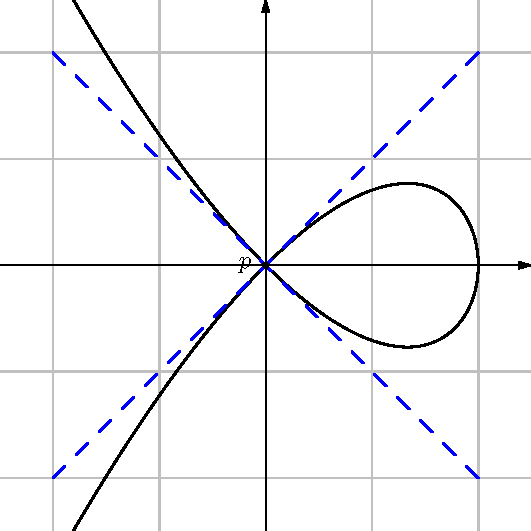
\includegraphics[scale=0.65]{fig-03.pdf}
    \caption{普通奇点, 两条切线}
    \label{fig:ordinary}
\end{figure}
\end{exmp}

\begin{exmp}[非普通奇点]
\label{exmp:non-ordinary}
设代数曲线 $C$ 的仿射方程为 $y^2 - x^3 = 0$,
则 $p = (0,0)$ 为 $C$ 的二重非普通奇点,
两条切线重合(都是 $y = 0$).
见 \cref{fig:non-ordinary} 如下:
\begin{figure}[H]
    \centering
    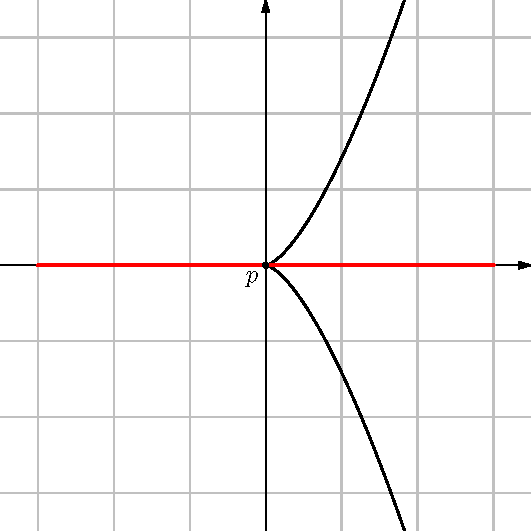
\includegraphics[scale=0.65]{fig-02.pdf}
    \caption{非普通奇点, 切线重合}
    \label{fig:non-ordinary}
\end{figure}
\end{exmp}

\section{Riemann 面及其拓扑}

\begin{defin}[Riemann 面]
\label{defin:2.4}
一个 \textbf{Riemann 面}是指 一个 \textit{连通的 Hausdorff} 空间 $X$,
以及 $X$ 的一个开覆盖 $\{U_\alpha\}$
和一族映射 $z_\alpha: U_\alpha \to \CC$, 称为\textbf{局部坐标系}, 使得
\begin{enumerate}[label=(\arabic*)]
    \ii 每个 $z_\alpha$ 把 $U_\alpha$ 同胚的映到 $\CC$ 的开子集 $z_\alpha(U_\alpha)$;
    \ii 若 $U_\alpha \cap U_\beta \ne \varnothing$, 则\textbf{转移函数}
    \[z_\beta\circ z_\alpha^{-1}: z_\alpha(U_\alpha\cap U_\beta) \to z_\beta(U_\alpha\cap U_\beta)\]
    是双全纯的(i.e., 是一个可逆的全纯函数并且逆也是全纯的).
\end{enumerate}
\end{defin}

和光滑流形类似, Riemann 面就是局部来看都是 $\CC$ 中开集的拓扑空间,
我们可以类似地定义复流形, 而 Riemann 面正是一维复流形.
类似于光滑流形之间的光滑映射, 我们可以定义复流形之间的全纯映射,
并且可以讨论两个复流形是否全纯同构.

\begin{exmp}[Riemann 球面]
\label{exmp:sphere}
射影直线 $\CP^1 = \{[\xi_0:\xi_1]:\xi_0,\xi_1 \in \CC\text{ 不同时为 0}\}$,
扩充复平面 $\ol{\CC} = \CC\cup \{\infty\}$,
以及 $\RR^3$ 中的单位球面 $S$ 是全纯同构的 Riemann 面, 称为 Riemann 球面.
设 $L$ 是 \cref{exmp:line} 中的直线,
注意到对 $[x:y] \in \CP^1$,
存在唯一的 $z$ 使得 $[z:x:y] \in L$,
通过这样的方式, 我们可以把 $\CP^2$ 中的直线都与 $\CP^1$ 等同起来.
\end{exmp}

\begin{exmp}[复射影平面]
\label{exmp:complex-manifold}
$\CP^2$ 是二维复流形. 对任意相同次数的齐次多项式 $F_0, F_1$,
$[\xi_0:\xi_1:\xi_2] \mapsto [F_0(\xi_0,\xi_1,\xi_2),F_1(\xi_0,\xi_1,\xi_2)]$
都是二维复流形 $\CP^2$ 到一维复流形 $\CP^1$ 的全纯映射.
\end{exmp}

\begin{exmp}[复环面]
\label{exmp:torus}
设 $w_1, w_2 \in \CC$ 是 $\RR$-线性无关的, 则它们决定了 $\CC$ 中一个格
\[\Lambda \defeq \{m_1w_1 + m_2w_2: m_1,m_2 \in \ZZ\} \cong \ZZ \oplus \ZZ,\]
格 $\Lambda$ 作为 $\CC$ 的子集有离散拓扑.
在 $\CC$ 中引入等价关系 $\sim$ 使得 $z \sim z' \iff z - z' \in \Lambda$,
得到的商空间 $\CC/\Lambda$ 是 Riemann 面, 称为复环面.
\end{exmp}

因为 $\CC \cong \RR^2$, 并且全纯映射总是光滑的,
所以一个 Riemann 面 $X$ 还能看作一个二维光滑流形,
并且由全纯映射满足 Cauchy-Riemann 方程知,
全纯映射还是保定向的(Jacobi 矩阵行列式 $> 0$),
所以这个二维光滑流形还是可定向的.
如果我们进一步假定 $X$ 还是紧致的,
则由拓扑学中的闭曲面分类定理\footnote{\cite{topo}, 第三章第四节}知,
$X$ 的拓扑被其亏格 $g$ 唯一决定.
注意到此时亏格 $g$ 被 $X$ 的另一个拓扑不变量
欧拉示性数 $\chi(X)$ 唯一决定,
它们的关系是:
\begin{equation}
\label{eq:genus-euler-relation}
\chi(X) = 2 - 2g.
\end{equation}
\cref{exmp:sphere} 和 \cref{exmp:torus} 中的 Riemann 球面和复环面
分别是亏格为 $0, 1$(相应的, 欧拉示性数为 $2, 0$)的 Riemann 面.

\section{Riemann 面之间的映射}
现在假设 $f: X \to Y$ 是 Riemann 面之间的一个非常值全纯映射.

\begin{lem}
\label{lem:surjective}
当 $X$ 是紧致的时候, $f$ 总是满射. 特别的, $Y$ 也是紧致的.
\end{lem}

\begin{proof}
因为紧集的像紧致, 且 $Y$ 作为 Hausdorff 空间, 它的紧致子集必为闭的,
所以 $f(X)$ 在 $Y$ 中闭.
另一方面, 全纯映射总是开映射, 所以 $f(X)$ 在 $Y$ 中开,
由连通性知只能是 $f(X) = Y$.
\end{proof}

\begin{prop}[分歧指标]
\label{prop:ramification-index}
设 $p \in X, q \in Y$ 满足 $f(p) = q$.
则存在 $p,q$ 的局部坐标系 $(U,z), (V,w)$ 使得
$z(p) = w(q) = 0$ 且在这个局部坐标系下 $f$ 形如 $w = f(z) = z^\mu, \mu \in \ZZ_{>0}$.
进一步, 正整数 $\mu$ 与局部坐标系的选取无关,
称为 $f$ 在 $p$ 处的\textbf{分歧指标}, 记为 $\nu_f(p)$,
$p,q$ 分别称为 ramification point 和 branch point.
\end{prop}

\begin{proof}
先任取局部坐标系 $(U',z'), (V,w)$ 使得 $z'(p) = w(q) = 0$,
在这个局部坐标系下 $f$ 形如
\[w = f(z') = (z')^n\cdot h(z'),\]
其中 $n \in \ZZ_{>0}, h(z')$ 是一全纯函数满足 $h(0) \ne 0$.
因为 $h(0) \ne 0$,
所以局部存在全纯函数 $r(z')$ 使得 $r(z')^n = h(z')$(这一点可由广义二项式定理看出),
于是适当的缩小 $U', V$ 后, 我们有 $f(z') = (z'r(z'))^n$.
因为 $r(0) \ne 0, z'r(z')$ 的幂级数展开中 $1$ 次项系数非零,
这意味着存在局部坐标系 $(U,z)$ 使得 $z = z'r(z')$,
在这个局部坐标看, $f$ 形如 $f(z) = z^n$.

设 $(U_1,z_1), (V_1, w_1)$ 是另一组满足条件的局部坐标系,
则存在可逆全纯函数 $\varphi, \psi$ 使得 $z = \varphi(z_1), w_1 = \psi(w)$,
于是 $f$ 在这组新局部坐标系下形如
$w_1 = \psi(w) = \psi(z^n) = \psi(\varphi(z_1)^n)$,
因为 $\varphi, \psi$ 都是可逆的, 所以它们的幂级数展开中一次项系数非零,
由此知 $n$ 是最小的正整数使得
$\psi(\varphi(z_1)^n)$ 幂级数展开中 $n$ 次项系数非零,
这就证明了 $n$ 与局部坐标系的选取无关.
\end{proof}

\Cref{lem:surjective} 告诉我们对任意 $q \in Y$,
存在 $p \in X$ 使得 $f(p) = q$.
\Cref{prop:ramification-index} 告诉我们存在 $p,q$ 的局部坐标系 $U,V$
以及正整数 $\mu = \nu_f(p)$ 使得
$f$ 在这组局部坐标系下形如
\begin{equation}
\label{eq:ramification-local-representation}
w = f(z) = z^\mu, \quad z \in U, w \in V.
\end{equation}
于是: $f^{-1}(0) = 0$,
对任意 $w \in V, w \ne 0, f^{-1}(w)$ 是 $U$ 中 $\mu$ 个不同的点.
换句话说, $f$ 是 $U\setminus \{0\}$ 到 $V\setminus \{0\}$ 的一个 $\mu$ 对 $1$ 的映射:
$f(z) = f(\omega z) = \cdots = f(\omega^{\mu - 1}z)$,
其中 $\omega$ 为 $\mu$ 次单位根.
于是我们有下述推论:

\begin{cor}
\label{cor:preimage-finite}
对任意 $q \in Y, f^{-1}(q)$ 作为 $X$ 的子空间有离散拓扑.
特别的, 当 $X$ 紧致的时候, $f^{-1}(q)$ 为有限集.
\end{cor}

\begin{prop}
\label{prop:ramification-point-finite}
$f$ 在 $U$ 中除 $p$ 外的点处都不分歧,
换句话说, $X$ 中的所有分歧点是离散的.
特别的, 当 $X$ 紧致的时候, 只有有限多个分歧点.
\end{prop}

\begin{proof}
假设对 $p \in U, q \in V, f(p) = q, f$ 在 $p$ 处分歧,
即 $\mu = \nu_f(p) \ge 2$, 则 $f$ 在 $U\setminus \{p\}$ 上是 $\mu$ 对 $1$ 的.
对 $q' \in V\setminus \{q\}$,
设 $p_1,\cdots, p_\mu$ 为 $X$ 中满足 $f(p_1) = \cdots = f(p_\mu) = q'$ 的 $\mu$ 个点.
对每个 $p_i$, 我们考虑 $f$ 在 $p_i$ 处的分歧情况:
存在 $p_i$ 的邻域 $U_i \subseteq U$ 以及 $q'$ 的邻域 $V' \subseteq V$,
使得 $f$ 在 $U_i\setminus \{p_i\}$ 上是 $\nu_f(p_i)$ 对 $1$ 的.
利用 Hausdorff 性质, 我们还可以适当缩小这些 $U_i$ 使得它们两两不交.
现在任取 $\tilde{q} \in V'\setminus \{q'\}$,
则一方面我们有 $\abs{f^{-1}(\tilde{q})\cap U} \ge \sum_{i=1}^\mu \nu_f(p_i)$,
另一方面, 因为 $f$ 在 $U\setminus \{p\}$ 上是 $\mu$ 对 $1$ 的,
所以 $\abs{f^{-1}(\tilde{q})\cap U} = \mu$,
这就推出 $\nu_f(p_i) = 1$.
\end{proof}

\begin{defin}[除子]
\label{defin:divisor}
Riemann 面 $X$ 上的\textbf{除子} $D$ 是一个形式和:
\[D = m_1p_1 + \cdots + m_lp_l,\]
其中 $m_j \in \ZZ, p_j \in X, j = 1,\cdots, l$.
称 $\sum_{j=1}^l m_j$ 为除子 $D$ 的次数, 记为 $\deg D$.
除子之间有自然的加法运算,
$X$ 上所有除子在这个运算下构成一个 Abel 群,
称为 $X$ 的除子群, 记为 $\Div(X)$.
显然 $\deg: \Div(X) \to \ZZ$ 是一个群同态.
\end{defin}

下面总是假设 Riemann 面 $X, Y$ 紧致.

\begin{exmp}[除子的拉回]
\label{exmp:divisor-pullback}
我们可以用全纯映射把 $Y$ 中的除子拉回到 $X$ 中:
设 $q$ 为 $Y$ 中一点, 则 $q$ 也可视作 $Y$ 的一个除子,
定义
\begin{equation}
\label{eq:divisor-pullback}
f^*(q) \defeq \sum_{p \in f^{-1}(q)}\nu_f(p)\cdot p.
\end{equation}
\cref{cor:preimage-finite} 保证了右边实际上是有限和,
所以 $f^*(q) \in \Div(X)$, 再作线性延拓,
我们便有群同态 $f^*: \Div(Y) \to \Div(X)$.
\end{exmp}

\begin{exmp}[分歧除子]
\label{exmp:ramification-divisor}
称
\begin{equation}
\label{eq:ramification-divisor}
R_f \defeq \sum_{p \in X}(v_f(p) - 1)p \in \Div(X)
\end{equation}
为全纯映射 $f$ 的\textbf{分歧除子}.
注意 \cref{prop:ramification-point-finite} 保证了 $R_f$ 是有限和.
\end{exmp}

对任意 $q \in Y$, 定义
\[\Phi(q) = \deg f^*(q) = \sum_{p \in f^{-1}(q)}\nu_f(p).\]

\begin{prop}
$\Phi: Y \to \ZZ$ 是局部常值的.
\end{prop}

\begin{proof}
考虑 $f$ 在所有使得 $f(p) = q$ 的点 $p \in X$ 处的分歧情况.
存在 $q$ 的开邻域 $V$, 还有各 $p$ 点处的开邻域 $U_p$,
使得 $f^{-1}(V) = \bigcup_p U_p$,
且 $f$ 局部地看是 $U_p\setminus \{p\}$ 到 $V\setminus \{q\}$ 的 $\nu_f(p)$ 对 $1$ 映射.
于是, 对所有的 $q' \in V\setminus \{q\}, f^{-1}(q') \cap U_p$ 为 $U_p$ 中 $\nu_f(p)$ 个点,
并且由 \cref{prop:ramification-point-finite} 知这 $\nu_f(p)$ 个点都不是分歧点,
故
\[\sum_{p' \in f^{-1}(q') \cap U_p} \nu_f(p') = \nu_f(p),\]
所以
\[\Phi(q') = \sum_{p' \in f^{-1}(q')}\nu_f(p') = \sum_{p \in f^{-1}(q)}\sum_{p' \in f^{-1}(q') \cap U_p} \nu_f(p') = \sum_{p \in f^{-1}(q)}\nu_f(p) = \Phi(q).\]
\end{proof}

\begin{cor}
$\Phi: Y \to \ZZ$ 是常值映射.
\end{cor}

\begin{proof}
局部常值告诉我们 $\Phi$ 是连续映射,
又因为 $Y$ 连通, 所以 $\Phi$ 必然是常值映射.
\end{proof}

\begin{defin}[全纯映射的次数]
\label{defin:mapping-degree}
任取 $q\in Y$, 称 $\Phi(q)$ 为全纯映射 $f$ 的\textbf{次数}, 记为 $\deg f$.
\end{defin}

\begin{prop}[Riemann-Hurwitz Formula]
\label{prop:Riemann-Hurwitz-Formula}
设 $f:X \to Y$ 是紧 Riemann 面之间的非常值全纯映射,
$R_f$ 为 $f$ 的分歧除子, 则有
\begin{equation}
\label{eq:Riemann-Hurwitz-Formula}
\deg f\cdot \chi(Y) = \chi(X) + \deg R_f.
\end{equation}
\end{prop}

\begin{proof}
见 \cite{textbook} 的第二章的定理 8.5.
\end{proof}

	% !TEX encoding = UTF-8 Unicode
\chapter{准备工作}
\label{chap:chap-3}

\fontsize{12bp}{14.4pt}

\section{局部不可约解析分支}

\begin{defin}
设 $\CC\{t\}, \CC\{x,y\}$ 是所有定义在 $0 \in \CC, (0,0) \in \CC^2$
附近的全纯函数 $z(t), \allowbreak f(x,y)$ 构成的集合, 即
\begin{align*}
    \CC\{t\} &= \bracketcur*{z(t) = \sum_{n=0}^\infty a_nt^n: z(t) \text{ 在
    $0$ 的一个邻域内收敛}},\\
    \CC\{x,y\} &= \bracketcur*{f(x,y) = \sum_{m,n=0}^\infty a_{m,n}x^my^n: f(x,y) \text{ 在
    $(0,0)$ 的一个邻域内收敛}}.
\end{align*}
\end{defin}

显然 $\CC\{t\},\CC\{x,y\}$ 有自然的加法和乘法结构, 因此构成环.
显然 $\CC\{t\}$ 中的单位(可逆元)为 $z(0) \ne 0$ 的全纯函数 $z(t)$,
$\CC\{x,y\}$ 中的单位为 $f(0,0) \ne 0$ 的全纯函数 $f(x,y)$.

\begin{defin}[Weierstrass 多项式]
\label{defin:weier-poly}
如果 $w \in \CC\{x\}[y]\subseteq \CC\{x,y\}$ 满足
\[w(x,y) = y^d + a_{d-1}(x)y^{d-1} + \cdots + a_0(x), \quad a_j(x) \in \CC\{x\},a_j(0) = 0, j = 0,\cdots, d - 1.\]
则称 $w$ 为一个(关于 $y$)的 \textbf{Weierstrass 多项式}.
\end{defin}

\begin{thm}[Weierstrass 预备定理]
\label{thm:Weierstrass-preparation}
设 $f(x,y) \in \CC\{x,y\}$ 满足 $f(0,y)$ 作为 $y$ 的多项式非零,
则在 $(0,0)$ 的一个充分小邻域内, $f(x,y)$ 可以被唯一表示成
\begin{equation}
    \label{eq:weierstrass-preparation}
    f(x,y) = u(x,y)\cdot w(x,y)
\end{equation}
其中 $u(x,y)$ 是 $\CC\{x,y\}$ 中的单位, $w(x,y) \in \CC\{x\}[y]$ 是一个 Weierstrass 多项式.
\end{thm}

\begin{proof}
见 \cite{textbook} 第二章的定理 4.5.
\end{proof}

Weierstrass 预备定理告诉我们, 局部来看(在 $(0,0)$ 的一个充分小邻域内),
$f(x,y)$ 的零点都由 Weierstrass 多项式贡献.

\begin{thm}
\label{thm:UFD}
$\CC\{t\}, \CC\{x\}[y], \CC\{x,y\}$ 都是唯一因子分解整环,
且 $f(x,y) \in \CC\{x\}[y] \subseteq \CC\{x,y\}$ 在小环 $\CC\{x\}[y]$ 中不可约
当且仅当它在大环 $\CC\{x,y\}$ 中不可约.
\end{thm}

\begin{proof}
见 \cite{textbook} 的第二章的推论 4.6.
\end{proof}

设 $z(t) \in \CC\{t\}$, 则 $z(t)$ 的分解情况为:
\begin{equation}
\label{eq:zt}
    z(t) = t^n\cdot h(t), \quad n \in \ZZ_{>0}, h(t) \in \CC\{t\}, h(0) \ne 0.
\end{equation}
也就是说 $\CC\{t\}$ 中的不可约元只有一个 $t$.

设 $f(x,y) \in \CC\{x,y\}$, 则 $f(x,y)$ 的分解情况为:
\begin{equation}
\label{eq:fxy}
    f(x,y) = x^n\cdot u(x,y)\cdot w_1(x,y)\cdots w_d(x,y),
\end{equation}
其中 $n \in \ZZ_{>0}, u(x,y) \in \CC\{x,y\}$ 为可逆元,
$w_j(x,y) \in \CC\{x\}[y], j = 1,\cdots, d$ 为不可约的 Weierstrass 多项式.

现在设 $C$ 是一条不可约代数曲线, 由仿射方程 $f(x,y)$ 给出,
并且不妨假设 $p = (0,0) \in C$, 即 $f(0,0) = 0$.
此时 $f(x,y)$ 虽然在 $\CC[x,y] = \CC[x][y]$ 中不可约,
但是如果我们视 $f(x,y)$ 为 $\CC\{x\}[y]$ 中的元素, 那么它未必是不可约的.
注意, 无论我们视 $f(x,y)$ 为 $\CC\{x\}[y]$ 中的元素还是 $\CC[x][y]$ 中的元素,
它的判别式 $\mathrm{disc}(f)$ 都是一样的,
而因为 $f(x,y)$ 在 $\CC[x][y]$ 中不可约, 所以 $\mathrm{disc}(f) \ne 0$,
这意味着 $f(x,y)$ 在 $\CC\{x\}[y]$ 中的分解也不会含有重因子.
于是 $f(x,y)$ 有形如 \cref{eq:fxy} 的分解(因为
$f(x,y)$ 不可约, 所以 \cref{eq:fxy} 中 $n = 0$):
\begin{equation}
\label{eq:analytic-decomposition}
f(x,y) = u(x,y)\cdot w_1(x,y)\cdots w_s(x,y).
\end{equation}
因为 $u(x,y)$ 为 $\CC\{x,y\}$ 中的可逆元, 即 $u(x,y) \ne 0$,
所以对 $(0,0)$ 的一个充分小的邻域
\[\Delta = \Delta(\rho,\varepsilon) \defeq\{(x,y) \in \CC^2: \abs{x} < \rho, \abs{y} < \varepsilon\},\]
$f(x,y)$ 的零点都由 $w_j(x,y)$ 贡献, 即
\[V(f) \cap \Delta = (V(w_1)\cap \Delta)\cup \cdots \cup (V(w_s)\cap \Delta).\]

\begin{defin}[局部不可约解析分支]
\label{defin:local-irre-component}
称 $V(w_j)\cap \Delta$ 为 $f(x,y)$ 在 $p = (0,0)$ 处的一个\textbf{局部不可约解析分支},
记为 $V_j$.
\end{defin}

现在假设 $w(x,y)$ 是一个不可约的 Weierstrass 多项式,
则 $\mathrm{disc}(w) \eqdef \mathcal{D}(x) \in \CC\{x\}$
是一个关于 $x$ 的在 $0$ 附近有定义的全纯函数.
注意到 $w(0,y) = y^k, k \in \ZZ_{>0}$.
\begin{itemize}
    \ii 若 $k = 1$, 则 $w(0,y)$ 无重根, 此时 $\mathcal{D}(0) \ne 0$;
    \ii 若 $k \ge 2$, 则 $w(0,y)$ 有重根, 此时 $\mathcal{D}(0) = 0$,
    但是 $\mathcal{D}(x)$ 作为一个解析函数, 零点是孤立的.
\end{itemize}
所以无论哪种情况, 我们总能选 $\rho$ 充分小,
使得 $\mathcal{D}(x) \ne 0, \forall\;0 < \abs{x} < \rho$.
同理, 可以选取 $\varepsilon$ 充分小,
使得对任意固定的 $x, \abs{x} < \rho$,
$w(x,y)$ 作为关于 $y$ 的多项式的 $k$ 个零点
$y_i(x), i = 1,\cdots, k$ 都满足模长 $\abs{y_i(x)} < \varepsilon$.
此时可以表
\[w(x,y) = y^k + a_{k-1}(x)y^{k-1} + \cdots + a_0(x) = (y-y_1(x))\cdots (y-y_k(x)).\]
由 $\rho$ 的选取, $\frac{\partial w}{\partial y}(x,y_i(x)) \ne 0$(否则
会推出 $\mathcal{D}(x) = 0$), 于是根据隐函数定理
$y_i(x)$ 在 $x$ 的一个充分小的邻域内全纯,
并且 $y_i(x)$ 能沿单连通区域
\[D \defeq \{x \in \CC: \abs{x} < \rho, x \notin [0,\rho)\} = \Delta(\rho)\setminus [0,\rho)\]
上的任意道路解析延拓.
利用 Riemann monodromy 定理,
我们可以把 $y_i(x)$全纯延拓成 $D$ 上的单值解析函数.
如果我们把 $y_i(x)$ 沿一条从 $[0,\rho)$ 下方并穿过
$[0,\rho)$ 的道路解析延拓,
得到的新的解析函数 $y_i^*(x)$ 依然满足 $w(x,y_i^*(x)) = 0$,
所以 $y_i^*(x)$ 在 $x$ 位于 $[0,\rho)$ 上方的取值
就是某个 $y_j(x), 1 \le j \le k$.
通过这样的方式, 我们得到了 $\{1,\cdots,k\}$ 的一个置换 $\sigma: i \mapsto j$.

\begin{figure}[H]
    \centering
    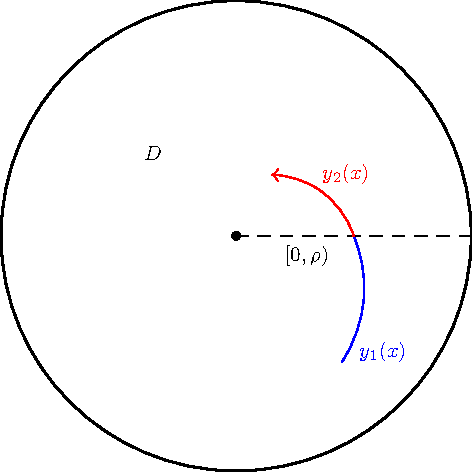
\includegraphics[scale = 0.8]{fig-05.pdf}
    \caption{$y_1(x)$ 沿一条穿过 $[0,\rho)$ 的道路解析延拓变成 $y_2(x)$.}
    \label{fig:analytic-continuation}
\end{figure}

\begin{prop}
\label{prop:irre-criterion}
一个 Weierstrass 多项式 $w(x,y)$ 不可约,
当且仅当 $\sigma$ 就是一个轮换.
\end{prop}

\begin{proof}
\footnote{\cite{textbook}, 第二章引理 5.6}我们先证明: 若 $\sigma$ 是一个轮换, 则
\begin{align*}
f(x,y) &= (y-y_1(x))\cdots (y-y_k(x)) = y^k + b_{k-1}(x)y^{k-1} + \cdots + b_0(x)\\
b_{k-1}(x) &= -(y_1(x) + \cdots + y_k(x))\\
\cdots &= \cdots\\
b_0(x) &= (-1)^ky_1(x)\cdots y_k(x)
\end{align*}
定义的 $f(x,y) \in \CC\{x\}[y]$.
事实上, 因为 $\sigma$ 是轮换,
所以系数 $b_0(x),\cdots, b_{k-1}(x)$ 在沿过 $[0,\rho)$ 的道路解析延拓后不变,
即这些系数都是 $\Delta(\rho)\setminus \{0\}$ 上的全纯函数,
显然它们还都是在 $0$ 的附近有界的(因为 $y_i(x)$ 满足模长 $<\varepsilon$),
这就证明了 $f(x,y) \in \CC\{x\}[y]$.

如果 $\sigma$ 分解成若干个不交轮换的乘积,
则给出了相应的 $w(x,y)$ 分解成若干个 Weierstrass 多项式的乘积,
反之亦然. 所以 $w(x,y)$ 不可约等价于 $\sigma$ 本身就是一个轮换.
\end{proof}

所以, 我们可以不妨假设置换 $\sigma$ 就是 $(12\cdots k)$,
也就是说: $y_i(x)$ 沿绕 $0$ 旋转 $m$ 周的道路延拓后成为 $y_{i+m}(x)$,
特别的 $y_i(x)$ 沿绕 $0$ 旋转 $k$ 周的道路延拓后不变.
在后文里, 如同 \cref{fig:analytic-continuation} 我们总是会假定 $y_i(x)$
沿一条穿过 $[0,\rho)$ 的道路解析延拓后变成 $y_{i+1}(x)$.

\begin{exmp}
$y^2 - x = (y-y_1(x))(y-y_2(x))$,
则每个 $y_i(x)$ 只是 $D$ 上的单值全纯函数,
而不是整个圆盘 $\Delta(\rho)$ 上单值全纯函数.
当我们让 $y_1(x)$ 沿过 $[0,\rho)$ 的道路延拓后,
就变成了 $y_2(x)$.
于是由 \cref{prop:irre-criterion} 知 $y^2 - x$ 在 $\CC\{x\}[y]$ 中不可约.
\end{exmp}

\begin{exmp}
考虑多项式 $f(x,y) = y^2 - x^2 + x^3 \in \CC[x,y] = \CC[x][y] \subseteq \CC\{x\}[y]$.
\begin{itemize}
    \ii $f(x,y)$ 在 $\CC[x,y]$ 中不可约:
    取 $\mathfrak{p} = (x-1)$ 为 $\CC[x]$ 中的素(极大)理想,
    显然 $x^3 - x^2 \notin \mathfrak{p}^2$,
    于是由 Eisenstein 判别法便知 $f(x,y)$ 不可约.
    \ii $f(x,y)$ 在 $\CC\{x\}[y]$ 中可约:
    事实上, $g(x) = x\cdot(1-x)^{\frac{1}{2}}$ 为定义在 $0$ 附近的解析函数(注意
    $(x-1)^{\frac{1}{2}}$ 可以利用广义二项式定理写出幂级数展开),
    满足 $g(x)^2 = x^2 - x^3$, 于是
    \[f(x,y) = (y-g(x))\cdot (y+g(x)).\]
\end{itemize}
当我们把注意力集中在 $x$ 充分小的时候(\cref{fig:local-seeing} 中为 $\abs{x} \le 0.25$),
$f(x,y)$ 近似为两条交于 $(0,0)$ 的曲线的并(这两条曲线分别由 $y = g(x)$ 和 $y = -g(x)$ 决定),
每一条曲线都是 $f(x,y)$ 在 $(0,0)$ 处的一个局部不可约解析分支.
\begin{figure}[H]
    \centering
    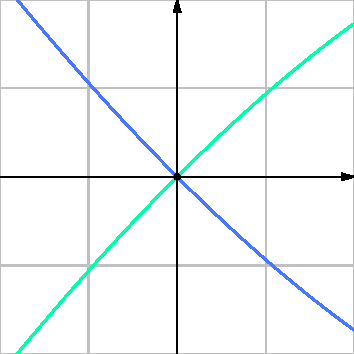
\includegraphics[scale = 1]{fig-04.pdf}
    \caption{局部地看 $f(x,y) = y^2 - x^2 + x^3 = 0$}
    \label{fig:local-seeing}
\end{figure}
\end{exmp}

\begin{rem}
在 $\CC[x,y]$ 中看相当于从整体来观察曲线,
在 $\CC\{x\}[y]$ 中看相当于观察 $\abs{x}$ 充分小时候的曲线,
在 $\CC\{x,y\}$ 中看相当于观察 $\abs{x},\abs{y}$ 同时充分小时候的曲线.
\cref{thm:UFD} 从这个角度来说就是:
曲线在 $\abs{x}$ 充分小时来看(相当于水平聚焦)不可约,
则即使再垂直聚焦也依然不可约.
\end{rem}

\section{正则化定理}

下述正则化定理把代数曲线 $C$ 和 Riemann 面联系了起来.
它可以看成是代数曲线 $C$ 的全纯参数表示,
其中参数取自 Riemann 面的局部坐标表示.
正则化定理的详细证明见 \cite{textbook}.

\begin{thm}[正则化定理]
\label{thm:normalization}
设 $C \subseteq \CP^2$ 为一条不可约代数曲线,
$S$ 是 $C$ 的所有奇点构成的集合,
在全纯同构的意义下,
存在唯一的紧 Riemann 面 $\tilde{C}$ 以及一个全纯映射
\[\sigma: \tilde{C} \to \CP^2\]
满足:
\begin{enumerate}[label=\normalfont(\arabic*)]
    \ii $\sigma(\tilde{C}) = C$;
    \ii 对任意 $p \in C, \sigma^{-1}(p)$ 为 Riemann 面 $\tilde{C}$ 中 $s$ 个不同的点,
    这里 $s$ 是 $p$ 处局部不可约解析分支的个数.
    \ii $\sigma: \tilde{C}\setminus\sigma^{-1}(S) \to C\setminus S$ 是单射.
\end{enumerate}
\end{thm}

\begin{thm}[局部正则化]
\label{thm:local-normalization}
设 $p = (0,0) \in C, \tilde{p} \in \sigma^{-1}(p)$,
正则化映射 $\sigma$ 可局部地表为:
\begin{itemize}
    \ii 若 $p$ 为光滑点, 则 $\frac{\partial f}{\partial x}(x,y)$
    和 $\frac{\partial f}{\partial y}(x,y)$ 不同时为 $0$,
    由隐函数定理知此时 $\sigma$ 为
    \[\sigma: x \mapsto (x,y(x)) \quad \text{or} \quad y \mapsto (x(y),y).\]
    \ii 若 $p$ 为奇点, $V$ 为 $p$ 处的一个局部不可约解析分支, 由 Weierstrass 多项式
    \begin{equation}
    \label{eq:irre-weierstrass}
    w(x,y) = y^l + a_1(x)y^{l-1} + \cdots + a_l(x) = \prod_{\mu=1}^l(y-y_\mu(x))
    \end{equation}
    给出. 则此时 $\sigma$ 为
    \begin{equation}
    \label{eq:local-normalization}
    \sigma: \Delta(\rho^{\frac{1}{l}}) \to V, \quad t\mapsto (t^l, \sigma_y(t)),
    \end{equation}
    \begin{center}
    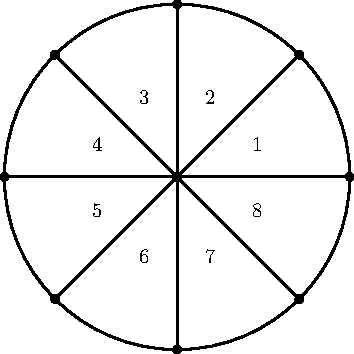
\includegraphics[scale=0.66]{fig-01.pdf}
    \end{center}
    这里我们将 $\Delta(\rho^{\frac{1}{l}})$ 等分为 $l$ 块扇形,
    当 $t$ 位于 $\Delta(\rho^{\frac{1}{l}})$ 中的第 $\mu$ 块扇形时,
    $\sigma(t)$ 的 $y$ 分量 $\sigma_y(t) = y_\mu(t^l)$.
    事实上, $\sigma$ 是 $\Delta(\rho^{\frac{1}{l}})$ 到 $V$ 的全纯双射,
    如果我们视 $V\setminus \{(0,0)\}$ 为一个 Riemann 面,
    则 $\sigma$ 还是 $\Delta(\rho^{\frac{1}{l}})\setminus \{0\}$ 到 $V\setminus \{(0,0)\}$
    的双全纯映射.
\end{itemize}
\end{thm}

\begin{rem}
因为 $y_\mu(x)$ 沿过 $[0,\rho)$ 的道路解析延拓时,
变成了 $y_{\mu + 1}(x)$,
这保证了局部正则化的定义是合理的.
对于 $p$ 是奇点的情形,
我们事实上得到了 $l$ 个不同的局部正则化,
每个局部正则化被 $t$ 位于第一块扇形时,
$\sigma(t)$ 的 $y$ 分量为哪个 $y_\mu(x)$ 唯一决定.
这 $l$ 个局部正则化两两之间只相差一个旋转(逆时针旋转若干次 $\frac{2\pi}{l}$).
\end{rem}

\begin{exmp}[直线的正则化]
\label{exmp:line-normalization}
设 $\ell: \alpha x - \beta y$ 为一条直线,
则它的局部正则化为 $\sigma: t \mapsto (\beta t, \alpha t)$.
\end{exmp}

\begin{exmp}
\label{exmp:non-ordinary-normalization}
代数曲线 $y^2 - x^3 = 0$ 就是一个在 $(0,0)$ 处的局部不可约解析分支(利用
\cref{prop:irre-criterion}),
局部正则化为 $\sigma: t \mapsto (t^2, t^3)$ 或 $t \mapsto (t^2, -t^3)$,
它们的 $y$ 分量差一个逆时针旋转 $\pi$.
\end{exmp}

\begin{exmp}
代数曲线 $y^2 - x^2 + x^3 = 0$ 在 $(0,0)$ 处有两个局部不可约解析分支:
\[y^2 - (x^2 - x^3) = (y - g(x))\cdot (y + g(x)),\]
局部正则化为 $\sigma: t \mapsto (t,g(t))$ 和 $\sigma: t \mapsto (t,-g(t))$.
\end{exmp}

\section{相交数, Bezout 定理}

\begin{defin}[order]
\label{defin:order}
设 $z(t)\in \CC\{t\}, \varphi(x,y) \in \CC\{x,y\}$.
\begin{itemize}
    \ii $z(t)$ 在 $0$ 处有幂级数展开
    \[z(t) = \sum_{n=0}^\infty \alpha_nt^n.\]
    称使得 $\alpha_n \ne 0$ 的最小非负整数 $n$ 为 $z(t)$ (关于 $t$)的 \textbf{order}.
    \ii $\varphi(x,y)$ 可以写成齐次部分的无穷和:
    \[\varphi(x,y) = \sum_{n=1}^\infty \varphi_n(x,y),\]
    其中 $\varphi_n(x,y)$ 为 $\varphi(x,y)$ 的 $n$ 次齐次部分.
    称使得 $\varphi_n(x,y) \ne 0$ 的最小非负整数 $n$
    为 $\varphi(x,y)$ 的 \textbf{order}.
\end{itemize}
\end{defin}

\begin{lem}
\label{lem:order-relation}
设 $w(x,y)$ 是一个由 \cref{eq:irre-weierstrass} 给出的不可约 Weierstrass 多项式,
$\sigma: t \mapsto (t^l, \sigma_y(t))$ 是它的局部正则化.
则我们有 $\sigma_y(t)$ 关于 $t$ 的 order
等于 $a_0(x)$ 关于 $x$ 的 order.
\end{lem}

\begin{proof}
注意事实上我们有 $l$ 个不同的局部正则化 $\sigma^1,\cdots, \sigma^l$,
其中当 $t$ 位于第 $1$ 块扇形时, $(\sigma^\mu)_y(t) = y_\mu(t^l)$.
这 $l$ 个局部正则化两两之间只相差一个旋转,
因而关于 $t$ 有相同的 order. 我们有
\begin{align*}
    \text{order of }(\sigma^1)_y(t) &= \frac{1}{l}\cdot \text{order of }\prod_{\mu=1}^{l}(\sigma^\mu)_y(t)\\
    &=\frac{1}{l}\cdot \text{order of }\prod_{\mu=1}^ly_\mu(t^l)\\
    &=\frac{1}{l}\cdot \text{order of }a_0(t^l)\\
    &=\text{order of }a_0(x).
\end{align*}
\end{proof}

在 \cref{exmp:non-ordinary-normalization} 中,
两个局部正则化分别为 $\sigma: t \mapsto (t^2, t^3)$ 和 $t \mapsto (t^2, -t^3)$,
而 $a_l(x) = a_2(x) = -x^3$, order 都为 $3$.

\begin{defin}[相交数]
\label{defin:intersection-number}
设 $f(x,y), h(x,y) \in \CC\{x\}[y]$ 为 Weierstrass 多项式,
\[V = \{(x,y) \in \CC^2: f(x,y) = 0\}, \quad W = \{(x,y) \in \CC^2: h(x,y) = 0\}\]
相交于 $p$(不妨设为 $p = (0,0)$).
如果 $f(x,y)$ 是不可约的,
设 $V$ 的局部正则化由 $\sigma: t \mapsto (t^l, \sigma_y(t))$ 给出,
定义 $V$ 和 $W$ 在 $p = (0,0)$ 处的\textbf{相交数}为 $h$ 用 $\sigma^*$ 拉回后关于 $t$ 的 order, 即
\[(V\cdot W)_p \defeq \text{order of }\sigma^*(h) = \text{order of }h(t^l,\sigma_y(t)).\]
对一般的由 $f(x,y) \in \CC[x][y]$ 定义的代数曲线,
在 $p = (0,0)$ 处 $V$ 分解为若干个局部不可约解析分支的并:
\[V = m_1V_1 + \cdots + m_lV_l,\]
即 $f(x,y)$ 在 $\CC\{x\}[y]$ 中分解成 $f = f_1^{m_1}\cdots f_l^{m_l}$,
每个 $V_i$ 是 $f_i$ 对应的局部不可约解析分支.
此时我们定义 $V$ 和 $W$ 在 $p$ 点处的相交数为
\[(V\cdot W)_p \defeq \sum_{j=1}^l m_j(V_j\cdot W)_p.\]
最后, 定义 $V$ 和 $W$ 的相交数为
\[(V \cdot W) \defeq \sum_{p \in V\cap W} (V\cdot W)_p.\]
\end{defin}

相交数的定义式中 $V, W$ 的地位是不对等的,
但是如果我们交换 $V, W$ 的位置得到的相交数是一样的(符合我们对相交的直观).

\begin{prop}[相交数的对称性]
$(V\cdot W)_p = (W\cdot V)_p$.
\end{prop}

\begin{proof}
设 $V,W$ 分别由 $f(x,y) = 0, h(x,y) = 0$ 定义, $p = (0,0)$.
我们只需证明结论对 $f(x,y), h(x,y)$ 都是不可约 Weierstrass 多项式时成立.
此时可表
\[f(x,y) = (y-y_1(x))\cdots (y-y_m(x)), \quad h(x,y) = (y-z_1(x))\cdots (y-z_n(x)),\]
其中 $y_i(x), z_j(x), 1 \le i \le m, 1 \le j \le n$
的定义同 \cref{eq:irre-weierstrass},
根据定义我们有
\begin{align*}
    (V\cdot W)_p &= \text{order of }h(t^m, y_i(t^m))\\
    &=\text{order of }\prod_{j=1}^n(y_i(t^m) - z_j(t^m)).
\end{align*}
同理我们有
\[(W\cdot V)_p = \text{order of }\prod_{i=1}^m(z_j(t^n) - y_i(t^n)). \]
但是
\begin{align*}
    \text{order of }\prod_{j=1}^n(y_i(t^m) - z_j(t^m)) &= \text{order of }h(t^m, y_i(t^m))\\
    &=\frac{1}{m}\text{order of }\prod_{i=1}^m h(t^m, y_i(t^m))\\
    &=\frac{1}{m}\text{order of }\prod_{i=1}^m\prod_{j=1}^n (y_i(t^m) - z_j(t^m))\\
    &=\frac{1}{mn}\text{order of }\prod_{i=1}^m\prod_{j=1}^n (y_i(t^{mn}) - z_j(t^{mn})).
\end{align*}
这里第二个等号相当于把 $h$ 用 $m$ 个不同的局部正则化拉回,
它们关于 $t$ 都有相同的 order.
完全类似地可得
\[\text{order of }\prod_{i=1}^m(z_j(t^n) - y_i(t^n))=\frac{1}{mn}\text{order of }\prod_{j=1}^n\prod_{i=1}^m (z_j(t^{mn}) - y_i(t^{mn})).\]
这就证明了 $(V\cdot W)_p = (W\cdot V)_p$.
\end{proof}

\begin{thm}[Bezout]
\label{thm:Bezout}
设 $C, E$ 为两条无公共分支的代数曲线, 即它们的齐次方程(仿射方程)无公共因子,
则有
\[(C\cdot E) = \sum_{p \in C\cap E}(C\cdot E)_p = \deg C \cdot \deg E.\]
\end{thm}

\begin{proof}
见 \cite{textbook} 第二章的定理 7.5.
注意 \cref{prop:line-bezout} 就是 $C,E$ 其中之一为直线的情形.
\end{proof}

现在设 $\varphi(x,y) \in \CC\{x\}[y]$ order 为 $n$,
\[\varphi(x,y) = \varphi_n(x,y) + \varphi_{n+1}(x,y) + \cdots.\]
因为 $\CC$ 是代数闭域, 它的 $n$ 次齐次部分 $\varphi_n(x,y)$ 可以分解成 $n$ 条直线的乘积:
\[\varphi_n(x,y) = (\alpha_1x - \beta_1y)\cdots (\alpha_nx - \beta_ny).\]
我们称这 $n$ 条直线为 $\varphi(x,y)$ 在 $(0,0)$ 处的切线.

\begin{prop}[相切的刻画]
\label{prop:tangent-chara}
设 $\ell: \alpha x - \beta y$ 是一条直线,
$\varphi(x,y) \in \CC\{x\}[y]$. 以下陈述等价:
\begin{enumerate}[label=\normalfont(\arabic*)]
    \ii $\ell$ 与 $\varphi(x,y)$ 相切.
    \ii $\ell$ 是 $\varphi(x,y)$ 的 $n$ 次齐次部分的因子.
    \ii $\text{order of }\varphi(\beta t,\alpha t) > n$.
    \ii $(\ell\cdot V(\varphi))_{(0,0)} > n$.
\end{enumerate}
\end{prop}

设 $C$ 是由仿射方程 $f(x,y)$ 给出的不可约代数曲线,
$f(x,y)$ 在 $\CC\{x\}[y]$ 中可进一步分解成 \cref{eq:analytic-decomposition}.
注意到我们有
\begin{equation}
\label{eq:order-sum-relation}
\sum_{j=1}^s \text{order of $w_j(x,y)$} = \text{order of $f(x,y)$}.
\end{equation}
而 order of $f(x,y)$ 正是 $p = (0,0)$ 的重数, 记为 $k$.
若我们表
\[w_j(x,y) = y^{l_j} + a_{l_j-1}^j(x)y^{l_j - 1} + \cdots + a_0^j(x),\]
则有 $l_j \ge n_j$, 以及 $k_j\defeq$ order of $a_0^j(x) \ge n_j$,
这里 $n_j \defeq \text{order of }w_j(x,y)$.
如果我们一开始就已经作了适当的旋转变换,
使得 $f(x,y)$ 在 $(0,0)$ 处的切线都不是 $x = 0$,
即 $y^k$ 出现在 $f(x,y)$ 的 $k$ 次齐次项中,
则此时必有 $l_j = n_j$(否则, 会推出 $y^k$ 的系数为 $0$).

\begin{prop}
\label{prop:only-one-tangent}
对每个局部不可约解析分支 $w_j(x,y)$, 在不计重数的意义下
有且只有一条直线 $\ell: \alpha x - \beta y$ 与它相切.
\end{prop}

\begin{proof}
设 $\sigma: t \mapsto (t^{l_j}, \sigma_y(t))$ 为 $w_j(x,y)$ 的局部正则化,
由 \cref{lem:order-relation} 知 $\sigma_y(t)$ 的 order 为 $k_j$, 于是可以表
\[\sigma_y(t) = \sum_{n = l_j}^\infty \alpha_nt^n,\quad \alpha_{k_j} \ne 0.\]
由相交数的对称性,
我们有 $\ell$ 与 $w_j(x,y)$ 相切
当且仅当 $(\ell \cdot V_j)_{(0,0)} > n_j = l_j$, 而
\[(\ell\cdot V_j)_{(0,0)} = \text{order of }\paren*{\alpha t^{l_j} - \beta \sum_{n=l_j}^\infty \alpha_nt^n}.\]
由此可见, $(\ell\cdot V_j)_{(0,0)} > l_j$ 当且仅当 $\alpha - \beta\alpha_{l_j} = 0$,
这就说明了与局部不可约解析分支 $w_j(x,y)$ 相切的直线有且只有
$y - \alpha_{l_j}x$ 这一条.
\end{proof}

\begin{cor}
\label{cor:ordinary}
设 $C$ 是一条不可约代数曲线, $p \in C$ 为 $k$ 重奇点,
则 $C$ 在 $p$ 处的局部不可约解析分支个数 $\le k$,
等号当 $p$ 为普通奇点时成立.
\end{cor}

\begin{proof}
第一个结论由 $w_j(0,0) = 0 \implies n_j \ge 1$, 再利用 \cref{eq:order-sum-relation} 推出.
当 $p$ 为普通奇点时,
在不计重数的意义下我们有 $k$ 条不同的切线.
另一方面, 注意到 $\ell$ 与 $C$ 在 $p$ 处相切,
当且仅当 $\ell$ 与某个局部不可约解析分支 $w_j(x,y)$ 相切,
于是由 \cref{prop:only-one-tangent} 知,
在不计重数的意义下, $C$ 在 $p$ 处至多有 $s$ 条不同的切线,
这推出 $k \le s$, 所以此时只能是 $k = s$.
\end{proof}

\begin{cor}
\label{cor:ordinary-normalization}
设 $p = (0,0)$ 是代数曲线 $C$ 的普通 $k$ 重奇点,
则 $C$ 在 $p$ 处的局部正则化可表为
\[\sigma: t \mapsto (t,y(t)) \quad \text{or} \quad \sigma: t \mapsto (x(t),t),\]
这里 $x(t), y(t) \in \CC\{t\}$.
\end{cor}

\begin{proof}
当 $p$ 是普通奇点时, 我们有 $k = s$,
以及 $n_j = 1, \forall\; j$.
注意 $n_j = 1$ 可以推出要么 $l_j = 1$, 要么 $k_j = 1$,
所以局部正则化 $\tau$
或者形如 $t \mapsto (t,y(t)), y(t) \in \CC\{t\}$,
或者形如 $t \mapsto (t^{l_j}, y(t))$, 其中 $y(t) \in \CC\{t\}$ 且 $y'(0) \ne 0$.
对于后者, 因为 $y'(0) \ne 0$, 利用反函数定理可以表 $t = \psi(y), \psi(y) \in \CC\{y\}$,
再命 $\sigma \defeq \tau\circ \psi$,
则 $\sigma(y) = \tau(t) = (\psi(y)^{l_j}, y) \eqdef (x(y), y)$.
\end{proof}

\begin{prop}
\label{prop:singularity-intersection-number}
设 $p = (0,0)$ 在代数曲线
\[V = \{(x,y) \in \CC^2:f(x,y) = 0\},\quad W = \{(x,y) \in \CC^2: h(x,y) = 0\}\]
中重数分别为 $k, m$, 则 $(V\cdot W)_p \ge km$.
\end{prop}

\begin{proof}
因为 $p = (0,0)$ 的重数分别为 $m, k$, 我们有
\[f(x,y) = f_k(x,y) + f_{k+1}(x,y) + \cdots, \quad h(x,y) = h_{m}(x,y) + h_{m+1}(x,y) + \cdots.\]
其中 $f_k(x,y), h_m(x,y)$ 分别为 $f,h$ 的 $k,m$ 次齐次部分.
$f(x,y)$ 可以进一步分解成同 \cref{eq:analytic-decomposition},
对每个局部不可约解析分支 $w_j(x,y)$, 我们有 $l_j \ge n_j, k_j \ge n_j$,
并且由 \cref{lem:order-relation} 知 $\sigma_y(t)$ 的 order $= k_j \ge n_j$,
这里 $\sigma$ 是 $w_j(x,y)$ 在 $p$ 处的局部正则化.
于是 order of $\sigma^*(h) = h(t^{l_j},\sigma_y(t)) \ge n_j\cdot m$,
故 $(V\cdot W)_p = \sum_{j=1}^s n_j\cdot m = km$.
\end{proof}


    % !TEX encoding = UTF-8 Unicode
\chapter{亏格公式}
\label{chap:chap-4}

\fontsize{12bp}{14.4pt}

设 $C\subseteq \CP^2$ 是一条次数为 $d$ 的不可约代数曲线,
$f(x,y)$ 是它的仿射方程,
$S$ 为 $C$ 的所有奇点构成的集合, 奇点 $p \in S$ 的重数记为 $m(p)$.
$\sigma: \tilde{C} \to C$ 是它的正则化,
$g = g(\tilde{C})$ 为 Riemann 的亏格.

\section{普通奇点的情形}

\begin{thm}[普通奇点的亏格公式]
\label{thm:genus-formula-ordinary}
假如 $C$ 的所有奇点都是普通奇点, 则
\begin{equation}
\label{eq:genus-formula-ordinary}
g = \frac{1}{2}(d-1)(d-2) - \sum_{p \in S}\frac{1}{2}m(p)(m(p) - 1) = \binom{d-1}{2} - \sum_{p \in S}\binom{m(p)}{2}.
\end{equation}
\end{thm}

我们先说明存在适当的坐标变换, 使得:
\begin{enumerate}[label=(\alph*)]
    \ii $L_\infty$ 与 $C$ 交于 $d$ 个不同的点.
    即 $L_\infty$ 在每个交点处的相交数都是 $1$,
    从而这 $d$ 个点都不是奇点(c.f. \cref{prop:singularity-intersection-number}),
    并且 $L$ 也不是 $C$ 的切线.
    \ii 奇点处的任意一条切线都不经过 $[0:0:1]$.
    \ii $[0:0:1] \notin C$.
\end{enumerate}

考虑另一条曲线 $E$, 由仿射方程 $\frac{\partial f(x,y)}{\partial y} = 0$ 定义.
一方面, 由 Bezout 定理我们有
\[(C\cdot E) = d(d-1).\]
下面我们将从另一个角度来计算 $C$ 和 $E$ 的相交数.

考虑 $C \subseteq \CP^2$ 到 $x$ 轴的投影
$\pi: [\xi_0:\xi_1:\xi_2]\mapsto [\xi_0:\xi_1:0]$.
注意映射 $\pi$ 实际上就是把 $\CP^2$ 中任意一点,
与 $[0:0:1]$ 连线再交直线 $\xi_2 = 0$ 得到的交点.
从仿射的角度来看, $\pi$ 就是往 $x$ 轴的投影, 即 $\pi: (x,y) \mapsto x$.
将直线 $\xi_2 = 0$ 与 $\CP^1$ 等同起来,
从 $\pi$ 的表达式容易看出这是复流形之间的全纯映射,
于是我们得到了 Riemann 面之间的全纯映射 $h\defeq \pi\circ \sigma: \tilde{C} \to \CP^1$.
\[\begin{tikzcd}
	{\tilde{C}} &&& C & {\mathbb{CP}^2} \\
	\\
	&&& {\mathbb{CP}^1}
	\arrow["\sigma", from=1-1, to=1-4]
	\arrow[hook, from=1-4, to=1-5]
	\arrow["\pi", from=1-4, to=3-4]
	\arrow["h"', from=1-1, to=3-4]
\end{tikzcd}\]

\begin{claim}
    $\deg h =$ 代数曲线 $C$ 的次数 $d$.
\end{claim}

事实上, 设 $\mathrm{disc}(f) \eqdef \mathcal{D}(x) \in \CC[x]$,
任取 $x_0 \in \CC$ 使得 $\mathcal{D}(x_0) \ne 0$,
则 $f(x_0,y) = 0$ 关于 $y$ 有 $d$ 个不同的解,
对应 $C$ 上 $d$ 个不同的点 $(x_0,y_i) \eqdef p_i, 1 \le i \le d$.
注意到这 $d$ 个点相当于直线 $x = x_0$ 与 $C$ 相交,
每个点处的相交数都只能恰好是 $1$,
由此便知它们都不是奇点(c.f. \cref{prop:singularity-intersection-number}),
并且每个点处的切线都不垂直于 $x$ 轴(即切线恰好为 $x = x_0$),
即 $\frac{\partial f(x,y)}{\partial y}|_{p_i} \ne 0$.
所以 $p_i$ 附近 $\sigma$ 可局部地表为 $x \mapsto (x,y(x)) \implies h$
可局部地表为 $h(x) = x$.
这就证明了 $h^{-1}(x_0)$ 是 $\tilde{C}$ 中 $d$ 个不同的点,
并且 $h$ 在每个点处的分歧指标都为 $1$, 所以 $\deg h = d$.

\begin{claim}
设 $\tilde{p} \in \tilde{C}, \sigma(\tilde{p}) = p$.
若 $p \in S$ 为 $C$ 的奇点, 则 $\tilde{p}$ 不是 $h$ 的分歧点.
\end{claim}

由 \cref{cor:ordinary-normalization} 知,
奇点 $p$ 附近的局部正则化为 $\sigma: t \mapsto (t,y(t))$
或 $t \mapsto (x(t),t)$.
对于前者, $h$ 局部来看形如 $h(t) = t$, 显然不是分歧的.
对于后者, $h$ 局部来看形如 $h(t) = x(t)$,
因为我们一开始已经假定了奇点处的切线都不经过 $[0:0:1]$,
即奇点处的切线都不垂直于 $x$ 轴,
所以 $x(t)$ 幂级数展开中的一次项系数非 $0$,
这就说明了此时 $h$ 依然不是分歧的.

$C$ 与 $E$ 的交点可以分为两类,
一类是光滑点, 一类是奇点,
显然任意奇点都是 $C$ 与 $E$ 的交点.

\begin{claim}
$C$ 与 $E$ 在奇点 $p$ 处的相交数为 $m(p)(m(p) - 1)$.
\end{claim}

不妨设 $p = (0,0)$, 记 $n = m(p)$. 首先我们可表
\[f(x,y) = f_n(x,y) + f_{n+1}(x,y) + \cdots, \quad f_n(x,y) \ne 0\]
以及
\[\frac{\partial f(x,y)}{\partial y} = g_{n-1}(x,y) + g_n(x,y) + \cdots, \quad g_j(x,y) = \frac{\partial f_{j+1}(x,y)}{\partial y}\]
为齐次部分的和.
因为 $p$ 是普通奇点, 由 \cref{cor:ordinary} 知
$f(x,y)$ 恰有 $n$ 个局部不可约解析分支,
于是我们只需证明:
对每一个局部不可约解析分支 $V_j$ 我们有 $(V_j\cdot E)_p = m(p) - 1 = n - 1$.
与前面讨论一样, 由 \cref{cor:ordinary-normalization} 知,
$V_j$ 的局部正则化为
\[t \mapsto (t,y(t)),\qquad y(t) = \alpha_1t + \alpha_2t^2 + \cdots,\]
或
\[t \mapsto (x(t),t) \qquad x(t) = \beta_1t + \beta_2t^2 + \cdots.\]
对于前者 $y - \alpha_1x$ 为 $V_j$ 的切线,
对于后者 $x - \beta_1y$ 为 $V_j$ 的切线,
我们暂时假定 $V_j$ 的局部正则化为第一种情形,
此时要说明 $(V_j\cdot E)_p = n - 1$, 只需说明
\[\frac{\partial f_n}{\partial y}(t,y(t)) = g_{n-1}(t,y(t)) \ne 0.\]
注意到
\[g_{n-1}(t,y(t)) = g_{n-1}(t,\alpha_1t+\alpha_2t^2 + \cdots) = t^{n-1}g_{n-1}(1,\alpha_1 + \alpha_2t+\cdots),\]
因为 $p$ 是普通奇点, $x \ndivides f_n(x,y)$, $p$ 处的 $n$ 条切线互不相同,
所以这 $n$ 条切线在 $f_n(x,y)$ 中的分解重数为 $1$,
故 $V_j$ 的切线 $y - \alpha_1x$ 不是 $g_{n-1}(x,y)$ 的因子,
于是我们有 $g_{n-1}(1,\alpha_1) \ne 0$.
这就证明了 $g_{n-1}(t,y(t))$ 的 order 为 $n - 1$,
同理可证 $V_j$ 的局部正则化为第二种情形时,
$(V_j\cdot E)_p = n - 1$ 也成立.

\begin{claim}
设 $C$ 与 $E$ 交于光滑点 $p$, 设 $\tilde{p} = \sigma^{-1}(p)$,
则 $C$ 与 $E$ 在 $p$ 处的相交数为 $\nu_h(\tilde{p}) - 1$.
\end{claim}

因为 $p$ 为光滑点, 且 $p \in E$, 所以
\[\restriction{\frac{\partial f(x,y)}{\partial x}}_p \ne 0.\]
于是 $p$ 附近的局部正则化为 $y \mapsto (x(y),y)$.
注意到我们有
\[0 = \frac{\partial f(x(y),y)}{\partial x}\cdot x'(y) + \frac{\partial f(x(y),y)}{\partial y},\]
由此可得
\[\text{order of }\frac{\partial f(x(y),y)}{\partial y} = \text{order of }x'(y) = \text{order of }x(y) - 1 = \nu_h(\tilde{p}) - 1.\]

综上, 我们得到了
\begin{align*}
d(d-1) &= \sum_{p\in C\cap E}(C\cdot E)_p\\
&= \sum_{p' \in (C\cap E)\setminus S}(C\cdot E)_{p'} + \sum_{p \in S}(C\cdot E)_p\\
&= \deg R_h + \sum_{p \in S}m(p)(m(p) - 1).
\end{align*}
最后再利用 Riemann-Hurwitz 公式(c.f. \cref{prop:Riemann-Hurwitz-Formula}),
\[\deg R_h = \deg h\cdot \chi(\CP^1) - \chi(\tilde{C}) = 2d - 2 + 2g,\]
便可得到亏格公式 \cref{eq:genus-formula-ordinary}.

\section{非普通奇点的情形}

非普通奇点的一个典型例子是 $y^2 - x^3 = 0$,
注意到 $[a:b]\mapsto [a^3:ab^2:b^3]$ 便是该曲线的正则化,
所以亏格应为 $g(\CP^1) = 0$.

现在我们考虑奇点的切线有重合的情形, 与之前不同,
此时若 $\tilde{p} \in \tilde{C}$ 是 $h$ 的分歧点,
则有可能出现 $\sigma(\tilde{p})$ 是 $C$ 的奇点.
以 $y^2 - x^3 = 0$ 为例, 在 $(0,0)$ 处只有一个局部不可约分支,
所以只有一个 $\tilde{p} \in \tilde{C}$ 使得 $\sigma(\tilde{p}) = (0,0)$.
另一方面, $\sigma$ 在 $\tilde{p}$ 处的局部正则化为 $t \mapsto (t^2, t^3)$,
由此可见 $h$ 在 $\tilde{p}$ 处的分歧指标为 $2$,
分歧除子 $R_h$ 在 $\tilde{p}$ 处的系数为 $1$.
再注意到 $f(x,y)$ 与 $\frac{\partial f(x,y)}{\partial y} = 2y$ 在 $(0,0)$ 处的相交数为
$\text{order of }2t^3 = 3$, 所以成立
\[d(d-1) - \deg R_h = 3 - 1 = 2,\]
这个 $2$ 来自于 $\tilde{p}$ 对分歧除子的贡献为 $1$,
但是对相交数的贡献却为 $3$, 两者相差了 $2$.
类似的方法可以知道, 对于 $y^2 - x^5 = 0$, 成立
\[d(d-1) - \deg R_h = 5 - 1 = 4.\]
那么对于一般的情形,
\begin{equation}
\label{eq:genus-formula-what}
d(d-1) - \deg R_h = \text{什么东西呢?}
\end{equation}

和普通奇点的情形一样, 若 $\sigma(\tilde{p})$ 为光滑点,
则 $\tilde{p}$ 对相交数的贡献和对分歧除子 $R_h$ 系数的贡献一致,
所以我们只需分析使得 $\sigma(\tilde{p})$ 为奇点的那些 $\tilde{p}$.

假设 $p = (0,0)$ 为 $C$ 的奇点, 重数为 $k$,
并且该奇点处有 $s = s(p)$ 个局部不可约解析分支,
则 $\sigma^{-1}(p)$ 为 $\tilde{C}$ 中 $s$ 个不同的点,
记为 $p_1,\cdots, p_s$, 每个 $p_j$ 对应的局部不可约解析分支为 $w_j(x,y)$.

若 $w_j(x,y)$ 的 order $n_j = l_j$,
则此时 $h$ 在 $p_j$ 可局部地表为 $h(t) = t^{l_j}$,
所以 $p_j$ 对 $\deg R_h$ 的贡献为 $l_j - 1 = n_j - 1$.
注意 $p_j$ 对相交数的贡献就是 $w_j(x,y)$ 与 $\frac{\partial f(x,y)}{\partial y}$ 的相交数,
记此相交数为 $I_j$,
则 $p_j$ 对 \cref{eq:genus-formula-what} 右边的贡献为 $I_j - n_j + 1$.
于是, 一般情形的亏格公式为
\begin{equation}
\label{eq:genus-formula-general}
g = \frac{1}{2}(d-1)(d-2) - \frac{1}{2}\sum_{p\in S}\sum_{j=1}^{s(p)}(I_j - n_j + 1).
\end{equation}
普通奇点的时候就是 \cref{eq:genus-formula-general} 中
$s(p) = m(p), I_j = m(p) - 1, n_j = 1$.
注意 $I_j$ 的取值依赖于奇点的复杂程度,
不能像普通奇点的情形一样, 简单依赖于奇点的重数 $m(p)$.
比如对于 $y^2 - x^{2m+1} = 0, m \in \ZZ_{>0}$,
$p = (0,0)$ 都是 $m(p) = 2$ 重奇点, $s(p) = 1, n_j = 2$,
但 $I_j = 2m + 1$.

\section{非普通奇点的另外一种处理方法}

数学中一种常见的处理问题的方法就是划归,
把新的问题转化为已经解决好的问题.
在 \cite{notes} 中, 我们考虑对曲线 $C$ 作适当的变换,
得到曲线 $D$, 使得 $C$ 的非普通奇点在变换之后成为了新曲线 $D$ 的普通奇点.

考虑变换 $T: [x:y:z]\mapsto [yz:xz:xy]$,
注意当 $xyz \ne 0$ 时, $T^2: [x:y:z]\mapsto [x^2yz:xy^2z:xyz^2] = [x:y:z]$,
由此可见 $T$ 是 $U \defeq \CP^2\setminus V(xyz)$ 上的一个全纯同构. 定义
\begin{equation}
\label{eq:psuedo-genus}
g^*(C) \defeq \binom{d-1}{2} - \sum_{p \in S}\binom{m(p)}{2}.
\end{equation}
于是对于只有普通奇点的代数曲线 $C, g^*(C) = g(C)$.
最后, 我们还需要找出 $g^*(D)$ 和 $g^*(C)$ 之间的关系.

\begin{lem}
\label{lem:pseudo-genus-always-non-negative}
对任意不可约代数曲线$C, g^*(C)$ 总是非负的.
\end{lem}

\begin{proof}
\footnote{\cite{notes}, 命题 1}
和亏格公式的证明一样, 我们考虑另一条代数曲线 $E$,
由仿射方程 $\frac{\partial f(x,y)}{\partial y} = 0$ 定义.
一方面由 Bezout 定理知 $(C\cdot E) = d(d-1)$.
另一方面, 对 $C$ 中任意重数为 $m$ 的点,
它在 $E$ 中的重数至少为 $m - 1$,
利用 \cref{prop:singularity-intersection-number} 便有
$d(d-1) \ge \sum m(m-1)$, 从而
\[r\defeq \frac{1}{2}(d+2)(d-1)-\sum_{p \in C\cap D}\frac{1}{2}m(p)(m(p) - 1)\ge 0.\]
设 $S^d$ 为所有 $d$ 次齐次多项式 $F(\xi_0,\xi_1,\xi_2)$ 构成的线性空间,
显然 $\dim S^d = \frac{1}{2}(d+2)(d+1)$.
注意 $S^d$ 中相差常数倍的两个齐次多项式实际代表同一条代数曲线,
所以次数为 $d$ 的代数曲线构成了 $\frac{1}{2}d(d+3)$ 维线性空间.
要使得某一点的重数为 $m$, 相当于给齐次多项式的系数增加 $\frac{1}{2}m(m+1)$ 个线性约束(比如,
若 $[1:0:0]$ 的重数为 $m$, 则我们要求 $\xi_1^i\xi_2^j, i+j < m$ 项的系数都为 $0$).
设 $G$ 是一个次数为 $d-1$ 的代数曲线,
满足对任意 $p \in C, m(p) \ge 2, p$ 为 $G$ 中的 $m(p)-1$ 重点,
并且 $G$ 与 $C$ 还有额外 $r$ 个公共点.
这样的 $G$ 总是存在的, 因为 $\frac{1}{2}(d-1)(d+2) - \sum\frac{1}{2}m(m-1) - r \ge 0$.
另一方面, 对 $F,G$ 用 Bezout 定理我们有 $(F\cdot G) = d(d-1) \ge \sum m(m-1) + r$,
由此便得 $\frac{1}{2}(d-1)(d-2) \ge \sum\frac{1}{2}m(m-1)$.
\end{proof}

\begin{lem}
\label{lem:transformation-property}
设 $F(\xi_0,\xi_1,\xi_2)$ 为 $n$ 次齐次多项式,
无一次因子 $\xi_0, \xi_1, \xi_2$.
设 $P,Q,R$ 分别为 $[0:0:1], [0:1:0], [1:0:0]$,
重数分别为 $a,b,c$.
定义
\begin{equation}
\label{eq:transformation}
\tilde{F}(\xi_0,\xi_1,\xi_2) \defeq \frac{F(\xi_1\xi_2, \xi_0\xi_2, \xi_0\xi_1)}{\xi_0^c\cdot\xi_1^b\cdot\xi_2^a}.
\end{equation}
\begin{enumerate}[label=\normalfont(\roman*)]
    \ii $\tilde{F}$ 为 $2n-a-b-c$ 次齐次多项式,
    并且 $\tilde{F}$ 再变换一次就变回原来的 $F$.
    \ii $P,Q,R$ 在代数曲线 $V(\tilde{F})$ 中的重数分别为
    $n-b-c,n-a-c,n-a-b$.
    \ii $F$ 不可约当且仅当 $\tilde{F}$ 不可约.
\end{enumerate}
\end{lem}

\begin{proof}
\footnote{\cite{notes}, 命题 2} (i) $\tilde{F}$ 的次数为 $2n-a-b-c$ 是显然的.
因为 $P$ 的重数为 $a$,
所以 $F$ 中 $\xi_2$ 的最高次数为 $n-a$, 所以我们有
\begin{align*}
F(\xi_0,\xi_1,\xi_2) &= F_a(\xi_0,\xi_1)\xi_2^{n-a} + \cdots + F_{n}(\xi_0,\xi_1),\\
F(\xi_1\xi_2,\xi_0\xi_2,\xi_1\xi_2) &= F_a(\xi_1\xi_2,\xi_0\xi_2)(\xi_0\xi_1)^{n-a} + \cdots + F_{n}(\xi_1\xi_2,\xi_0\xi_2),
\end{align*}
其中 $F_i(\xi_0,\xi_1)$ 为 $i$ 次齐次多项式.
由此可见 $\tilde{F}$ 也不含一次因子 $\xi_2$,
换句话说, $\tilde{F}$ 就是 $F(\xi_1\xi_2,\xi_0\xi_2,\xi_0\xi_1)$ 再约去所有一次因子,
所以 $\tilde{F}$ 再作一次变换就变回原来的 $F$.

(ii) 我们有
\[\tilde{F}(\xi_0,\xi_1,\xi_2) = \sum_{i=0}^{n-a}F_{a+i}(\xi_1,\xi_0)\xi_0^{n-a-c-i}\xi_1^{n-a-b-i}\xi_2^i,\]
即关于 $\xi_2$ 的最高次数为 $n-a$,
所以 $P$ 在 $V(\tilde{F})$ 中的重数为 $2n-a-b-c-(n-a) = n-b-c$.
同理可得 $Q,R$ 在 $V(\tilde{F})$ 中的重数.

(iii) 显然 $F$ 的任意分解都给出了 $\tilde{F}$ 的一个分解, 反之亦然.
\end{proof}

设 $C = V(F), D = V(\tilde{F}), P$ 为 $C$ 中重数为 $k$ 的奇点.
进行适当的坐标变换, 使得:
\begin{enumerate}[label=(\alph*)]
    \ii 直线 $\xi_0 = 0, \xi_1 = 0$ 都与 $C$ 交于 $P$ 以及 $P$ 之外 $n-k$ 个不同的点.
    \ii $Q,R \notin C$.
    \ii 直线 $\xi_2 = 0$ 与 $C$ 交于 $n$ 个不同的点.
\end{enumerate}

\begin{lem}
\label{lem:singularity-become-ordinary}
在上述条件下, $D$ 的奇点及奇点的重数为:
\begin{enumerate}[label=\normalfont(\roman*)]
    \ii 在 $U$ 中 $C$ 与 $D$ 全纯同构, 因而奇点有一一对应关系,
    互相对应的奇点性状完全相同(重数一样, 普通奇点对应普通奇点, 非普通奇点对应非普通奇点).
    \ii $P,Q,R$ 都是 $D$ 的普通奇点.
    \ii $D\cap \{\xi_0 = 0\} = \{P,Q\}, D\cap \{\xi_1 = 0\} = \{P,R\}$.
    \ii 除点 $Q,R$ 外, $D$ 与直线 $\xi_2 = 0$ 的相交数为 $k$.
    换句话说, $D$ 与直线 $\xi_2 = 0$ 在 $Q,R$ 处的相交数都恰好为 $n-k$.
\end{enumerate}
\end{lem}

\begin{proof}
\footnote{\cite{notes}, 引理 3}
(i) 显然.

(ii) 由 \cref{lem:transformation-property} 知 $\tilde{F}$ 的次数为 $2n - k$,
$P,Q,R$ 的重数分别为 $n, n-k, n-k$.
注意 $P$ 的 $n$ 次齐次项为 $F_{n}(\xi_1,\xi_0)$,
结合条件 (c) 便知 $P$ 点处的 $n$ 条切线互异,
故 $P$ 为普通奇点.
同理, 考察 $Q,R$ 的 $n-k$ 次齐次项,
再结合条件 (a) 便知 $Q,R$ 也为普通奇点.

(iii) 因为 $P,Q$ 的重数分别为 $n, n-k$,
由 \cref{prop:singularity-intersection-number} 知
$D$ 与 $\xi_0 = 0$ 在 $P,Q$ 处的相交数分别至少为 $n,n-k$,
再由 Bezout 定理便知 $D\cap \{\xi_0 = 0\}$ 只有 $P,Q$ 两点.
同理可证 $D\cap \{\xi_1 = 0\} = \{P,R\}$.

(iv) 事实上, 若表
\[F(\xi_0,\xi_1,\xi_2) = \sum_{i=0}^n G_i(\xi_1,\xi_2)\xi_0^{n-i},\]
其中 $G_i$ 为 $i$ 次齐次多项式, 则
\[\tilde{F}(\xi_0,\xi_1,\xi_2) = \sum_{i=0}^n G_i(\xi_2,\xi_1)\xi_1^{n-i}\xi_2^{n-k-i}\xi_0^i.\]
于是 $\xi_2 = 0$ 与 $\tilde{F}$ 在 $R$ 处的相交数为
\[\text{order of }\restriction{G_n(y,x)y^{-k}}_{y=0} \le n - k,\]
结合 $R$ 的重数为 $n-k$ 及 \cref{prop:singularity-intersection-number} 便可得证.
\end{proof}

\begin{cor}
\label{cor:pseudo-genus-relation}
我们有 $g^*(D) = g^*(C) - \sum_{r}\binom{\ol{m}(r)}{2}$,
这里 $\ol{m}(r)$ 为 $r\in (D\cap V(\xi_2))\setminus \{Q,R\}$ 在 $D$ 中的重数.
\end{cor}

\begin{proof}
\footnote{\cite{notes}, 推论 4} 我们有
\[g^*(C) = \binom{n-1}{2} - \binom{k}{2} - \sum_q\binom{m(q)}{2},\]
其中 $\sum_q$ 为对所有 $C$ 中的奇点 $q \ne P$ 求和. 以及
\begin{align*}
g^*(D) &= \binom{2n-k-1}{2} - \binom{n}{2} - 2\cdot\binom{n-k}{2} - \sum_r \binom{\ol{m}(r)}{2}\\
&=\binom{n-1}{2} - \binom{k}{2} - \sum_r\binom{\ol{m}(r)}{2},
\end{align*}
其中 $\sum_r$ 为对所有 $D$ 中的奇点 $r \notin \{P,Q,R\}$ 求和.
于是
\[g^*(C) - g^*(D) = \sum_r\binom{\ol{m}(r)}{2} - \sum_q\binom{m(q)}{2}.\]
由 \cref{lem:singularity-become-ordinary} 的 (i) 知
我们只需计算 $q,r \in \CP^2\setminus U = V(\xi_0)\cup V(\xi_1)\cup V(\xi_2)$ 的贡献.
由 (a),(c) 知这样的 $q$ 不存在,
由 \cref{lem:singularity-become-ordinary} 的 (iii) 和 (iv)
知这样的 $r \in D\cap V(\xi_2)$
\end{proof}

也就是说变换之后, $g^*$ 要么严格变小要么不变,
对于后者, 我们有 $\ol{m}(r) = 1$,
即 $\xi_2 = 0$ 与 $D$ 的除 $Q,R$ 外的交点都不是奇点,
此时非普通奇点的个数严格变小.
对于前者, 由 \cref{lem:pseudo-genus-always-non-negative} 知这样的情形只会发生有限多次.
于是, 经过若干次这样的变换之后, 我们便回到了所有奇点都是普通奇点的情形.

\begin{exmp}
对代数曲线 $\xi_0^3 = \xi_1^2\xi_2$ 作坐标变换
$(\xi_0,\xi_1,\xi_2) \mapsto (\xi_0+\xi_1,\xi_0-\xi_1,\xi_0+\xi_2)$,
我们有 $(\xi_0+\xi_1)^3 = (\xi_0-\xi_1)^2(\xi_0+\xi_2)$,
记这个齐次方程对应的曲线为 $C$,
则对应的 $D$ 的齐次方程为 $(\xi_1-\xi_0)^2\xi_1 = \xi_2(\xi_0^2 + 2\xi_0\xi_1 + 5\xi_1^2)$.
对新曲线 $D$ 而言, $[0:0:1]$ 变成了普通奇点.
\end{exmp}

    
    \appendix
    \printbibliography[heading = bibintoc]

	\backmatter
	% !TEX encoding = UTF-8 Unicode
\chapter{致谢}

首先我要感谢我的论文指导老师同时亦是我的课程老师蔡金星,
细致耐心地指导了我,
一学期的课程更是让我收获满满.
其次, 我要感谢我的朋友周昊天与萧浩梁,
感谢他们耐心地与我讨论一些我在写作过程中遇到的问题,
还有他们的宝贵建议.

I hereby leave this record \textbf{as my} firm achievement.

	% 需添加二维码
	% Copyright (c) 2008-2009 solvethis
% Copyright (c) 2010-2017,2021 Casper Ti. Vector
% Copyright (c) 2021 Kurapica
% Copyright (c) 2021 iofu728
% All rights reserved.
%
% Redistribution and use in source and binary forms, with or without
% modification, are permitted provided that the following conditions are
% met:
%
% * Redistributions of source code must retain the above copyright notice,
%   this list of conditions and the following disclaimer.
% * Redistributions in binary form must reproduce the above copyright
%   notice, this list of conditions and the following disclaimer in the
%   documentation and/or other materials provided with the distribution.
% * Neither the name of Peking University nor the names of its contributors
%   may be used to endorse or promote products derived from this software
%   without specific prior written permission.
%
% THIS SOFTWARE IS PROVIDED BY THE COPYRIGHT HOLDERS AND CONTRIBUTORS "AS
% IS" AND ANY EXPRESS OR IMPLIED WARRANTIES, INCLUDING, BUT NOT LIMITED TO,
% THE IMPLIED WARRANTIES OF MERCHANTABILITY AND FITNESS FOR A PARTICULAR
% PURPOSE ARE DISCLAIMED. IN NO EVENT SHALL THE COPYRIGHT HOLDER OR
% CONTRIBUTORS BE LIABLE FOR ANY DIRECT, INDIRECT, INCIDENTAL, SPECIAL,
% EXEMPLARY, OR CONSEQUENTIAL DAMAGES (INCLUDING, BUT NOT LIMITED TO,
% PROCUREMENT OF SUBSTITUTE GOODS OR SERVICES; LOSS OF USE, DATA, OR
% PROFITS; OR BUSINESS INTERRUPTION) HOWEVER CAUSED AND ON ANY THEORY OF
% LIABILITY, WHETHER IN CONTRACT, STRICT LIABILITY, OR TORT (INCLUDING
% NEGLIGENCE OR OTHERWISE) ARISING IN ANY WAY OUT OF THE USE OF THIS
% SOFTWARE, EVEN IF ADVISED OF THE POSSIBILITY OF SUCH DAMAGE.

{
	\ctexset{section = {
		format+ = {\centering}, beforeskip = {40bp}, afterskip = {15bp}
	}}
	\specialchap{北京大学学位论文原创性声明和使用授权说明}

	% 学校书面要求本页面不要页码,但在给出的 Word 模版中又有页码。
	% 此处以学校书面要求为准。
	\thispagestyle{empty}
	\mbox{}\vspace*{-3em}
	\section*{原创性声明}

	本人郑重声明:
	所呈交的学位论文,是本人在导师的指导下,独立进行研究工作所取得的成果。
	除文中已经注明引用的内容外,
	本论文不含任何其他个人或集体已经发表或撰写过的作品或成果。
	对本文的研究做出重要贡献的个人和集体,均已在文中以明确方式标明。
	本声明的法律结果由本人承担。
	\vskip 3em
	\rightline{%
		论文作者签名:\raisebox{-0.3em}{\includegraphics[scale=0.018]{signature-student.png}}\hspace{2.5em}%
	}
    \medskip
    \rightline{
		日期:2021 年 5 月 25 日%
    }

	\section*{%
		学位论文使用授权说明\\[-0.33em]
		%\textmd{\zihao{5}(必须装订在提交学校图书馆的印刷本)}%
	}

	本人完全了解北京大学关于收集、保存、使用学位论文的规定,即:
	\begin{itemize}
		\item 按照学校要求提交学位论文的印刷本和电子版本;
		\item 学校有权保存学位论文的印刷本和电子版,
			并提供目录检索与阅览服务,在校园网上提供服务;
		\item 学校可以采用影印、缩印、数字化或其它复制手段保存论文;
	\end{itemize}
	\vskip 3em
	\rightline{%
		论文作者签名:\raisebox{-0.3em}{\includegraphics[scale=0.018]{signature-student.png}}\hspace{0.5em}
        导师签名:\raisebox{-0.2em}{\includegraphics[scale=0.1]{signature-teacher.jpg}}%
	}
    \medskip
    \rightline{
		日期:2021 年 5 月 25 日%
    }

    % 若须排版二维码,请将二维码图片重命名为“barcode”,
    % 二维码内容为: 北京大学 xx学院 xx专业 xxx
    % 容错设置25%
    % 转为合适的图片格式,并放在当前目录下,然后去掉下面 2 行的注释。
    % \vfill\noindent
    % \includegraphics[height = 5em]{barcode}
}

% vim:ts=4:sw=4


\end{document}

% vim:ts=4:sw=4
